% TFL-TAGE-SC-L: 50-trace evaluation report.
% Build:  tectonic main.tex      (or: pdflatex main && bibtex main && pdflatex main && pdflatex main)
% Every number in the text is a \val{...} generated from the result CSVs by
% experiments/scripts/make_report_50trace.py (generated/values.tex); tables are in generated/.
\documentclass[11pt,a4paper]{article}
\usepackage[T1]{fontenc}
\usepackage{lmodern}
\usepackage{amsmath,amssymb}
\usepackage{graphicx}
\usepackage{booktabs}
\usepackage{longtable}
\usepackage{array}
\usepackage{xcolor}
\usepackage[margin=2.2cm]{geometry}
\usepackage{caption}
\usepackage{float}
\usepackage{microtype}
\usepackage{enumitem}
\usepackage[numbers,sort&compress]{natbib}
\usepackage[hidelinks]{hyperref}
\usepackage{url}
\setlist{itemsep=2pt,topsep=4pt}
\captionsetup{font=small,labelfont=bf}
% generated by experiments/scripts/make_report_50trace.py -- do not edit
\makeatletter
\newcommand{\val}[1]{\ifcsname val@#1\endcsname\csname val@#1\endcsname\else\errmessage{undefined report value #1}\fi}
\expandafter\def\csname val@n_traces\endcsname{50}
\expandafter\def\csname val@n_traces_agg\endcsname{50}
\expandafter\def\csname val@n_orig\endcsname{10}
\expandafter\def\csname val@n_add\endcsname{40}
\expandafter\def\csname val@n_int\endcsname{26}
\expandafter\def\csname val@n_fp\endcsname{24}
\expandafter\def\csname val@n_bench\endcsname{20}
\expandafter\def\csname val@n_runs\endcsname{350}
\expandafter\def\csname val@n_runs_ok\endcsname{350}
\expandafter\def\csname val@n_runs_failed\endcsname{0}
\expandafter\def\csname val@total_sim_hours\endcsname{176.0}
\expandafter\def\csname val@trace_gb\endcsname{16.06}
\expandafter\def\csname val@started\endcsname{2026-10-31 21:48}
\expandafter\def\csname val@finished\endcsname{2026-11-01 10:26}
\expandafter\def\csname val@bim_kb\endcsname{4.00}
\expandafter\def\csname val@bim_bits\endcsname{32,768}
\expandafter\def\csname val@bim_mean_ipc\endcsname{0.9065}
\expandafter\def\csname val@bim_gm_ipc\endcsname{0.7797}
\expandafter\def\csname val@bim_mpki\endcsname{9.334}
\expandafter\def\csname val@bim_median_mpki\endcsname{5.750}
\expandafter\def\csname val@bim_acc\endcsname{93.089}
\expandafter\def\csname val@bim_cacc\endcsname{91.476}
\expandafter\def\csname val@bim_speedup_bim\endcsname{+0.00}
\expandafter\def\csname val@bim_hours\endcsname{24.0}
\expandafter\def\csname val@bim_mean_wall_min\endcsname{28.8}
\expandafter\def\csname val@gsh_kb\endcsname{4.00}
\expandafter\def\csname val@gsh_bits\endcsname{32,782}
\expandafter\def\csname val@gsh_mean_ipc\endcsname{0.9825}
\expandafter\def\csname val@gsh_gm_ipc\endcsname{0.8330}
\expandafter\def\csname val@gsh_mpki\endcsname{4.619}
\expandafter\def\csname val@gsh_median_mpki\endcsname{2.529}
\expandafter\def\csname val@gsh_acc\endcsname{96.580}
\expandafter\def\csname val@gsh_cacc\endcsname{95.964}
\expandafter\def\csname val@gsh_speedup_bim\endcsname{+6.84}
\expandafter\def\csname val@gsh_hours\endcsname{24.6}
\expandafter\def\csname val@gsh_mean_wall_min\endcsname{29.5}
\expandafter\def\csname val@perc_kb\endcsname{3.98}
\expandafter\def\csname val@perc_bits\endcsname{32,624}
\expandafter\def\csname val@perc_mean_ipc\endcsname{1.0060}
\expandafter\def\csname val@perc_gm_ipc\endcsname{0.8508}
\expandafter\def\csname val@perc_mpki\endcsname{3.700}
\expandafter\def\csname val@perc_median_mpki\endcsname{1.748}
\expandafter\def\csname val@perc_acc\endcsname{97.260}
\expandafter\def\csname val@perc_cacc\endcsname{96.676}
\expandafter\def\csname val@perc_speedup_bim\endcsname{+9.13}
\expandafter\def\csname val@perc_hours\endcsname{24.8}
\expandafter\def\csname val@perc_mean_wall_min\endcsname{29.8}
\expandafter\def\csname val@hp_kb\endcsname{64.03}
\expandafter\def\csname val@hp_bits\endcsname{524,542}
\expandafter\def\csname val@hp_mean_ipc\endcsname{1.0539}
\expandafter\def\csname val@hp_gm_ipc\endcsname{0.8845}
\expandafter\def\csname val@hp_mpki\endcsname{1.922}
\expandafter\def\csname val@hp_median_mpki\endcsname{0.706}
\expandafter\def\csname val@hp_acc\endcsname{98.577}
\expandafter\def\csname val@hp_cacc\endcsname{98.244}
\expandafter\def\csname val@hp_speedup_bim\endcsname{+13.45}
\expandafter\def\csname val@hp_hours\endcsname{25.5}
\expandafter\def\csname val@hp_mean_wall_min\endcsname{30.6}
\expandafter\def\csname val@tage_kb\endcsname{46.84}
\expandafter\def\csname val@tage_bits\endcsname{383,674}
\expandafter\def\csname val@tage_mean_ipc\endcsname{1.0597}
\expandafter\def\csname val@tage_gm_ipc\endcsname{0.8877}
\expandafter\def\csname val@tage_mpki\endcsname{1.805}
\expandafter\def\csname val@tage_median_mpki\endcsname{0.464}
\expandafter\def\csname val@tage_acc\endcsname{98.663}
\expandafter\def\csname val@tage_cacc\endcsname{98.352}
\expandafter\def\csname val@tage_speedup_bim\endcsname{+13.86}
\expandafter\def\csname val@tage_hours\endcsname{25.6}
\expandafter\def\csname val@tage_mean_wall_min\endcsname{30.8}
\expandafter\def\csname val@tsl_kb\endcsname{58.14}
\expandafter\def\csname val@tsl_bits\endcsname{476,319}
\expandafter\def\csname val@tsl_mean_ipc\endcsname{1.0636}
\expandafter\def\csname val@tsl_gm_ipc\endcsname{0.8909}
\expandafter\def\csname val@tsl_mpki\endcsname{1.663}
\expandafter\def\csname val@tsl_median_mpki\endcsname{0.378}
\expandafter\def\csname val@tsl_acc\endcsname{98.769}
\expandafter\def\csname val@tsl_cacc\endcsname{98.481}
\expandafter\def\csname val@tsl_speedup_bim\endcsname{+14.27}
\expandafter\def\csname val@tsl_hours\endcsname{25.7}
\expandafter\def\csname val@tsl_mean_wall_min\endcsname{30.8}
\expandafter\def\csname val@prop_kb\endcsname{62.09}
\expandafter\def\csname val@prop_bits\endcsname{508,666}
\expandafter\def\csname val@prop_mean_ipc\endcsname{1.0641}
\expandafter\def\csname val@prop_gm_ipc\endcsname{0.8914}
\expandafter\def\csname val@prop_mpki\endcsname{1.628}
\expandafter\def\csname val@prop_median_mpki\endcsname{0.348}
\expandafter\def\csname val@prop_acc\endcsname{98.795}
\expandafter\def\csname val@prop_cacc\endcsname{98.512}
\expandafter\def\csname val@prop_speedup_bim\endcsname{+14.33}
\expandafter\def\csname val@prop_hours\endcsname{25.7}
\expandafter\def\csname val@prop_mean_wall_min\endcsname{30.9}
\expandafter\def\csname val@prop_minus_tsl_bits\endcsname{32,347}
\expandafter\def\csname val@prop_minus_tsl_kb\endcsname{3.95}
\expandafter\def\csname val@prop_minus_tsl_pct\endcsname{6.8}
\expandafter\def\csname val@hp_minus_prop_bits\endcsname{15,876}
\expandafter\def\csname val@best_ipc\endcsname{TFL-TAGE-SC-L}
\expandafter\def\csname val@prop_rank_ipc\endcsname{1}
\expandafter\def\csname val@best_mpki\endcsname{TFL-TAGE-SC-L}
\expandafter\def\csname val@prop_rank_mpki\endcsname{1}
\expandafter\def\csname val@best_acc\endcsname{TFL-TAGE-SC-L}
\expandafter\def\csname val@prop_rank_acc\endcsname{1}
\expandafter\def\csname val@best_mean_ipc\endcsname{TFL-TAGE-SC-L}
\expandafter\def\csname val@best_base\endcsname{TAGE-SC-L}
\expandafter\def\csname val@best_default\endcsname{Hashed perceptron}
\expandafter\def\csname val@vs_bim_pct_mpki\endcsname{82.56}
\expandafter\def\csname val@vs_bim_abs_mpki\endcsname{7.7064}
\expandafter\def\csname val@vs_bim_ipc\endcsname{+14.329}
\expandafter\def\csname val@vs_bim_meanipc\endcsname{+17.387}
\expandafter\def\csname val@vs_bim_acc_pp\endcsname{+5.706}
\expandafter\def\csname val@vs_bim_mpki_win\endcsname{49}
\expandafter\def\csname val@vs_bim_mpki_tie\endcsname{1}
\expandafter\def\csname val@vs_bim_mpki_loss\endcsname{0}
\expandafter\def\csname val@vs_bim_ipc_win\endcsname{47}
\expandafter\def\csname val@vs_bim_ipc_tie\endcsname{1}
\expandafter\def\csname val@vs_bim_ipc_loss\endcsname{2}
\expandafter\def\csname val@vs_bim_ipc_win_half\endcsname{42}
\expandafter\def\csname val@vs_bim_ipc_loss_half\endcsname{0}
\expandafter\def\csname val@vs_bim_best_trace\endcsname{654.roms\_s-842B}
\expandafter\def\csname val@vs_bim_best_pct\endcsname{+72.76}
\expandafter\def\csname val@vs_bim_worst_trace\endcsname{619.lbm\_s-2676B}
\expandafter\def\csname val@vs_bim_worst_pct\endcsname{-0.01}
\expandafter\def\csname val@vs_bim_bestm_trace\endcsname{654.roms\_s-842B}
\expandafter\def\csname val@vs_bim_bestm\endcsname{27.999}
\expandafter\def\csname val@vs_bim_worstm_trace\endcsname{649.fotonik3d\_s-1176B}
\expandafter\def\csname val@vs_bim_worstm\endcsname{0.0000}
\expandafter\def\csname val@vs_bim_top_trace\endcsname{654.roms\_s-842B}
\expandafter\def\csname val@vs_bim_top_share\endcsname{7.3}
\expandafter\def\csname val@vs_bim_pct_mpki_excl_top\endcsname{81.46}
\expandafter\def\csname val@vs_bim_median_ipc\endcsname{+10.582}
\expandafter\def\csname val@vs_bim_n_ipc_flat\endcsname{4}
\expandafter\def\csname val@vs_bim_n_ipc_gt0p1\endcsname{43}
\expandafter\def\csname val@vs_bim_n_ipc_ltm0p1\endcsname{0}
\expandafter\def\csname val@vs_gsh_pct_mpki\endcsname{64.76}
\expandafter\def\csname val@vs_gsh_abs_mpki\endcsname{2.9908}
\expandafter\def\csname val@vs_gsh_ipc\endcsname{+7.013}
\expandafter\def\csname val@vs_gsh_meanipc\endcsname{+8.309}
\expandafter\def\csname val@vs_gsh_acc_pp\endcsname{+2.214}
\expandafter\def\csname val@vs_gsh_mpki_win\endcsname{49}
\expandafter\def\csname val@vs_gsh_mpki_tie\endcsname{1}
\expandafter\def\csname val@vs_gsh_mpki_loss\endcsname{0}
\expandafter\def\csname val@vs_gsh_ipc_win\endcsname{48}
\expandafter\def\csname val@vs_gsh_ipc_tie\endcsname{1}
\expandafter\def\csname val@vs_gsh_ipc_loss\endcsname{1}
\expandafter\def\csname val@vs_gsh_ipc_win_half\endcsname{38}
\expandafter\def\csname val@vs_gsh_ipc_loss_half\endcsname{0}
\expandafter\def\csname val@vs_gsh_best_trace\endcsname{623.xalancbmk\_s-165B}
\expandafter\def\csname val@vs_gsh_best_pct\endcsname{+27.51}
\expandafter\def\csname val@vs_gsh_worst_trace\endcsname{619.lbm\_s-2676B}
\expandafter\def\csname val@vs_gsh_worst_pct\endcsname{-0.01}
\expandafter\def\csname val@vs_gsh_bestm_trace\endcsname{641.leela\_s-334B}
\expandafter\def\csname val@vs_gsh_bestm\endcsname{9.848}
\expandafter\def\csname val@vs_gsh_worstm_trace\endcsname{649.fotonik3d\_s-1176B}
\expandafter\def\csname val@vs_gsh_worstm\endcsname{0.0000}
\expandafter\def\csname val@vs_gsh_top_trace\endcsname{641.leela\_s-334B}
\expandafter\def\csname val@vs_gsh_top_share\endcsname{6.6}
\expandafter\def\csname val@vs_gsh_pct_mpki_excl_top\endcsname{65.38}
\expandafter\def\csname val@vs_gsh_median_ipc\endcsname{+4.820}
\expandafter\def\csname val@vs_gsh_n_ipc_flat\endcsname{3}
\expandafter\def\csname val@vs_gsh_n_ipc_gt0p1\endcsname{42}
\expandafter\def\csname val@vs_gsh_n_ipc_ltm0p1\endcsname{0}
\expandafter\def\csname val@vs_perc_pct_mpki\endcsname{56.01}
\expandafter\def\csname val@vs_perc_abs_mpki\endcsname{2.0727}
\expandafter\def\csname val@vs_perc_ipc\endcsname{+4.767}
\expandafter\def\csname val@vs_perc_meanipc\endcsname{+5.777}
\expandafter\def\csname val@vs_perc_acc_pp\endcsname{+1.535}
\expandafter\def\csname val@vs_perc_mpki_win\endcsname{49}
\expandafter\def\csname val@vs_perc_mpki_tie\endcsname{1}
\expandafter\def\csname val@vs_perc_mpki_loss\endcsname{0}
\expandafter\def\csname val@vs_perc_ipc_win\endcsname{48}
\expandafter\def\csname val@vs_perc_ipc_tie\endcsname{1}
\expandafter\def\csname val@vs_perc_ipc_loss\endcsname{1}
\expandafter\def\csname val@vs_perc_ipc_win_half\endcsname{33}
\expandafter\def\csname val@vs_perc_ipc_loss_half\endcsname{0}
\expandafter\def\csname val@vs_perc_best_trace\endcsname{603.bwaves\_s-1080B}
\expandafter\def\csname val@vs_perc_best_pct\endcsname{+18.97}
\expandafter\def\csname val@vs_perc_worst_trace\endcsname{619.lbm\_s-2676B}
\expandafter\def\csname val@vs_perc_worst_pct\endcsname{-0.01}
\expandafter\def\csname val@vs_perc_bestm_trace\endcsname{603.bwaves\_s-1080B}
\expandafter\def\csname val@vs_perc_bestm\endcsname{11.696}
\expandafter\def\csname val@vs_perc_worstm_trace\endcsname{649.fotonik3d\_s-1176B}
\expandafter\def\csname val@vs_perc_worstm\endcsname{0.0000}
\expandafter\def\csname val@vs_perc_top_trace\endcsname{603.bwaves\_s-1080B}
\expandafter\def\csname val@vs_perc_top_share\endcsname{11.3}
\expandafter\def\csname val@vs_perc_pct_mpki_excl_top\endcsname{53.05}
\expandafter\def\csname val@vs_perc_median_ipc\endcsname{+2.509}
\expandafter\def\csname val@vs_perc_n_ipc_flat\endcsname{5}
\expandafter\def\csname val@vs_perc_n_ipc_gt0p1\endcsname{40}
\expandafter\def\csname val@vs_perc_n_ipc_ltm0p1\endcsname{0}
\expandafter\def\csname val@vs_hp_pct_mpki\endcsname{15.29}
\expandafter\def\csname val@vs_hp_abs_mpki\endcsname{0.2939}
\expandafter\def\csname val@vs_hp_ipc\endcsname{+0.772}
\expandafter\def\csname val@vs_hp_meanipc\endcsname{+0.973}
\expandafter\def\csname val@vs_hp_acc_pp\endcsname{+0.218}
\expandafter\def\csname val@vs_hp_mpki_win\endcsname{46}
\expandafter\def\csname val@vs_hp_mpki_tie\endcsname{2}
\expandafter\def\csname val@vs_hp_mpki_loss\endcsname{2}
\expandafter\def\csname val@vs_hp_ipc_win\endcsname{45}
\expandafter\def\csname val@vs_hp_ipc_tie\endcsname{2}
\expandafter\def\csname val@vs_hp_ipc_loss\endcsname{3}
\expandafter\def\csname val@vs_hp_ipc_win_half\endcsname{24}
\expandafter\def\csname val@vs_hp_ipc_loss_half\endcsname{0}
\expandafter\def\csname val@vs_hp_best_trace\endcsname{638.imagick\_s-4128B}
\expandafter\def\csname val@vs_hp_best_pct\endcsname{+3.75}
\expandafter\def\csname val@vs_hp_worst_trace\endcsname{619.lbm\_s-2676B}
\expandafter\def\csname val@vs_hp_worst_pct\endcsname{-0.02}
\expandafter\def\csname val@vs_hp_bestm_trace\endcsname{641.leela\_s-602B}
\expandafter\def\csname val@vs_hp_bestm\endcsname{1.057}
\expandafter\def\csname val@vs_hp_worstm_trace\endcsname{644.nab\_s-9322B}
\expandafter\def\csname val@vs_hp_worstm\endcsname{0.0019}
\expandafter\def\csname val@vs_hp_top_trace\endcsname{641.leela\_s-602B}
\expandafter\def\csname val@vs_hp_top_share\endcsname{7.2}
\expandafter\def\csname val@vs_hp_pct_mpki_excl_top\endcsname{15.85}
\expandafter\def\csname val@vs_hp_median_ipc\endcsname{+0.435}
\expandafter\def\csname val@vs_hp_n_ipc_flat\endcsname{8}
\expandafter\def\csname val@vs_hp_n_ipc_gt0p1\endcsname{33}
\expandafter\def\csname val@vs_hp_n_ipc_ltm0p1\endcsname{0}
\expandafter\def\csname val@vs_tage_pct_mpki\endcsname{9.82}
\expandafter\def\csname val@vs_tage_abs_mpki\endcsname{0.1773}
\expandafter\def\csname val@vs_tage_ipc\endcsname{+0.413}
\expandafter\def\csname val@vs_tage_meanipc\endcsname{+0.417}
\expandafter\def\csname val@vs_tage_acc_pp\endcsname{+0.131}
\expandafter\def\csname val@vs_tage_mpki_win\endcsname{46}
\expandafter\def\csname val@vs_tage_mpki_tie\endcsname{3}
\expandafter\def\csname val@vs_tage_mpki_loss\endcsname{1}
\expandafter\def\csname val@vs_tage_ipc_win\endcsname{46}
\expandafter\def\csname val@vs_tage_ipc_tie\endcsname{3}
\expandafter\def\csname val@vs_tage_ipc_loss\endcsname{1}
\expandafter\def\csname val@vs_tage_ipc_win_half\endcsname{17}
\expandafter\def\csname val@vs_tage_ipc_loss_half\endcsname{0}
\expandafter\def\csname val@vs_tage_best_trace\endcsname{657.xz\_s-2302B}
\expandafter\def\csname val@vs_tage_best_pct\endcsname{+2.23}
\expandafter\def\csname val@vs_tage_worst_trace\endcsname{619.lbm\_s-2676B}
\expandafter\def\csname val@vs_tage_worst_pct\endcsname{-0.02}
\expandafter\def\csname val@vs_tage_bestm_trace\endcsname{627.cam4\_s-490B}
\expandafter\def\csname val@vs_tage_bestm\endcsname{1.076}
\expandafter\def\csname val@vs_tage_worstm_trace\endcsname{638.imagick\_s-824B}
\expandafter\def\csname val@vs_tage_worstm\endcsname{0.0003}
\expandafter\def\csname val@vs_tage_top_trace\endcsname{627.cam4\_s-490B}
\expandafter\def\csname val@vs_tage_top_share\endcsname{12.1}
\expandafter\def\csname val@vs_tage_pct_mpki_excl_top\endcsname{9.13}
\expandafter\def\csname val@vs_tage_median_ipc\endcsname{+0.145}
\expandafter\def\csname val@vs_tage_n_ipc_flat\endcsname{13}
\expandafter\def\csname val@vs_tage_n_ipc_gt0p1\endcsname{27}
\expandafter\def\csname val@vs_tage_n_ipc_ltm0p1\endcsname{0}
\expandafter\def\csname val@vs_tsl_pct_mpki\endcsname{2.09}
\expandafter\def\csname val@vs_tsl_abs_mpki\endcsname{0.0347}
\expandafter\def\csname val@vs_tsl_ipc\endcsname{+0.052}
\expandafter\def\csname val@vs_tsl_meanipc\endcsname{+0.049}
\expandafter\def\csname val@vs_tsl_acc_pp\endcsname{+0.026}
\expandafter\def\csname val@vs_tsl_mpki_win\endcsname{29}
\expandafter\def\csname val@vs_tsl_mpki_tie\endcsname{5}
\expandafter\def\csname val@vs_tsl_mpki_loss\endcsname{16}
\expandafter\def\csname val@vs_tsl_ipc_win\endcsname{30}
\expandafter\def\csname val@vs_tsl_ipc_tie\endcsname{5}
\expandafter\def\csname val@vs_tsl_ipc_loss\endcsname{15}
\expandafter\def\csname val@vs_tsl_ipc_win_half\endcsname{1}
\expandafter\def\csname val@vs_tsl_ipc_loss_half\endcsname{0}
\expandafter\def\csname val@vs_tsl_best_trace\endcsname{627.cam4\_s-490B}
\expandafter\def\csname val@vs_tsl_best_pct\endcsname{+1.17}
\expandafter\def\csname val@vs_tsl_worst_trace\endcsname{621.wrf\_s-6673B}
\expandafter\def\csname val@vs_tsl_worst_pct\endcsname{-0.01}
\expandafter\def\csname val@vs_tsl_bestm_trace\endcsname{627.cam4\_s-490B}
\expandafter\def\csname val@vs_tsl_bestm\endcsname{0.750}
\expandafter\def\csname val@vs_tsl_worstm_trace\endcsname{644.nab\_s-9322B}
\expandafter\def\csname val@vs_tsl_worstm\endcsname{0.0026}
\expandafter\def\csname val@vs_tsl_top_trace\endcsname{627.cam4\_s-490B}
\expandafter\def\csname val@vs_tsl_top_share\endcsname{43.2}
\expandafter\def\csname val@vs_tsl_pct_mpki_excl_top\endcsname{1.26}
\expandafter\def\csname val@vs_tsl_median_ipc\endcsname{+0.005}
\expandafter\def\csname val@vs_tsl_n_ipc_flat\endcsname{28}
\expandafter\def\csname val@vs_tsl_n_ipc_gt0p1\endcsname{7}
\expandafter\def\csname val@vs_tsl_n_ipc_ltm0p1\endcsname{0}
\expandafter\def\csname val@all50_bim_mpki\endcsname{9.334}
\expandafter\def\csname val@all50_bim_gm_ipc\endcsname{0.7797}
\expandafter\def\csname val@all50_bim_red\endcsname{82.56}
\expandafter\def\csname val@all50_bim_ipcimp\endcsname{+14.329}
\expandafter\def\csname val@all50_gsh_mpki\endcsname{4.619}
\expandafter\def\csname val@all50_gsh_gm_ipc\endcsname{0.8330}
\expandafter\def\csname val@all50_gsh_red\endcsname{64.76}
\expandafter\def\csname val@all50_gsh_ipcimp\endcsname{+7.013}
\expandafter\def\csname val@all50_perc_mpki\endcsname{3.700}
\expandafter\def\csname val@all50_perc_gm_ipc\endcsname{0.8508}
\expandafter\def\csname val@all50_perc_red\endcsname{56.01}
\expandafter\def\csname val@all50_perc_ipcimp\endcsname{+4.767}
\expandafter\def\csname val@all50_hp_mpki\endcsname{1.922}
\expandafter\def\csname val@all50_hp_gm_ipc\endcsname{0.8845}
\expandafter\def\csname val@all50_hp_red\endcsname{15.29}
\expandafter\def\csname val@all50_hp_ipcimp\endcsname{+0.772}
\expandafter\def\csname val@all50_tage_mpki\endcsname{1.805}
\expandafter\def\csname val@all50_tage_gm_ipc\endcsname{0.8877}
\expandafter\def\csname val@all50_tage_red\endcsname{9.82}
\expandafter\def\csname val@all50_tage_ipcimp\endcsname{+0.413}
\expandafter\def\csname val@all50_tsl_mpki\endcsname{1.663}
\expandafter\def\csname val@all50_tsl_gm_ipc\endcsname{0.8909}
\expandafter\def\csname val@all50_tsl_red\endcsname{2.09}
\expandafter\def\csname val@all50_tsl_ipcimp\endcsname{+0.052}
\expandafter\def\csname val@all50_prop_mpki\endcsname{1.628}
\expandafter\def\csname val@all50_prop_gm_ipc\endcsname{0.8914}
\expandafter\def\csname val@original10_bim_mpki\endcsname{9.884}
\expandafter\def\csname val@original10_bim_gm_ipc\endcsname{0.6239}
\expandafter\def\csname val@original10_bim_red\endcsname{69.19}
\expandafter\def\csname val@original10_bim_ipcimp\endcsname{+10.078}
\expandafter\def\csname val@original10_gsh_mpki\endcsname{6.153}
\expandafter\def\csname val@original10_gsh_gm_ipc\endcsname{0.6531}
\expandafter\def\csname val@original10_gsh_red\endcsname{50.50}
\expandafter\def\csname val@original10_gsh_ipcimp\endcsname{+5.159}
\expandafter\def\csname val@original10_perc_mpki\endcsname{5.384}
\expandafter\def\csname val@original10_perc_gm_ipc\endcsname{0.6620}
\expandafter\def\csname val@original10_perc_red\endcsname{43.43}
\expandafter\def\csname val@original10_perc_ipcimp\endcsname{+3.745}
\expandafter\def\csname val@original10_hp_mpki\endcsname{3.247}
\expandafter\def\csname val@original10_hp_gm_ipc\endcsname{0.6838}
\expandafter\def\csname val@original10_hp_red\endcsname{6.22}
\expandafter\def\csname val@original10_hp_ipcimp\endcsname{+0.433}
\expandafter\def\csname val@original10_tage_mpki\endcsname{3.295}
\expandafter\def\csname val@original10_tage_gm_ipc\endcsname{0.6827}
\expandafter\def\csname val@original10_tage_red\endcsname{7.58}
\expandafter\def\csname val@original10_tage_ipcimp\endcsname{+0.590}
\expandafter\def\csname val@original10_tsl_mpki\endcsname{3.072}
\expandafter\def\csname val@original10_tsl_gm_ipc\endcsname{0.6864}
\expandafter\def\csname val@original10_tsl_red\endcsname{0.85}
\expandafter\def\csname val@original10_tsl_ipcimp\endcsname{+0.058}
\expandafter\def\csname val@original10_prop_mpki\endcsname{3.046}
\expandafter\def\csname val@original10_prop_gm_ipc\endcsname{0.6868}
\expandafter\def\csname val@additional40_bim_mpki\endcsname{9.197}
\expandafter\def\csname val@additional40_bim_gm_ipc\endcsname{0.8243}
\expandafter\def\csname val@additional40_bim_red\endcsname{86.15}
\expandafter\def\csname val@additional40_bim_ipcimp\endcsname{+15.417}
\expandafter\def\csname val@additional40_gsh_mpki\endcsname{4.235}
\expandafter\def\csname val@additional40_gsh_gm_ipc\endcsname{0.8852}
\expandafter\def\csname val@additional40_gsh_red\endcsname{69.93}
\expandafter\def\csname val@additional40_gsh_ipcimp\endcsname{+7.481}
\expandafter\def\csname val@additional40_perc_mpki\endcsname{3.280}
\expandafter\def\csname val@additional40_perc_gm_ipc\endcsname{0.9059}
\expandafter\def\csname val@additional40_perc_red\endcsname{61.18}
\expandafter\def\csname val@additional40_perc_ipcimp\endcsname{+5.024}
\expandafter\def\csname val@additional40_hp_mpki\endcsname{1.590}
\expandafter\def\csname val@additional40_hp_gm_ipc\endcsname{0.9433}
\expandafter\def\csname val@additional40_hp_red\endcsname{19.93}
\expandafter\def\csname val@additional40_hp_ipcimp\endcsname{+0.856}
\expandafter\def\csname val@additional40_tage_mpki\endcsname{1.433}
\expandafter\def\csname val@additional40_tage_gm_ipc\endcsname{0.9479}
\expandafter\def\csname val@additional40_tage_red\endcsname{11.12}
\expandafter\def\csname val@additional40_tage_ipcimp\endcsname{+0.369}
\expandafter\def\csname val@additional40_tsl_mpki\endcsname{1.310}
\expandafter\def\csname val@additional40_tsl_gm_ipc\endcsname{0.9509}
\expandafter\def\csname val@additional40_tsl_red\endcsname{2.82}
\expandafter\def\csname val@additional40_tsl_ipcimp\endcsname{+0.051}
\expandafter\def\csname val@additional40_prop_mpki\endcsname{1.273}
\expandafter\def\csname val@additional40_prop_gm_ipc\endcsname{0.9514}
\expandafter\def\csname val@INT_bim_mpki\endcsname{12.003}
\expandafter\def\csname val@INT_bim_gm_ipc\endcsname{0.6554}
\expandafter\def\csname val@INT_bim_red\endcsname{77.14}
\expandafter\def\csname val@INT_bim_ipcimp\endcsname{+18.983}
\expandafter\def\csname val@INT_gsh_mpki\endcsname{7.169}
\expandafter\def\csname val@INT_gsh_gm_ipc\endcsname{0.7062}
\expandafter\def\csname val@INT_gsh_red\endcsname{61.73}
\expandafter\def\csname val@INT_gsh_ipcimp\endcsname{+10.426}
\expandafter\def\csname val@INT_perc_mpki\endcsname{5.674}
\expandafter\def\csname val@INT_perc_gm_ipc\endcsname{0.7310}
\expandafter\def\csname val@INT_perc_red\endcsname{51.65}
\expandafter\def\csname val@INT_perc_ipcimp\endcsname{+6.672}
\expandafter\def\csname val@INT_hp_mpki\endcsname{3.138}
\expandafter\def\csname val@INT_hp_gm_ipc\endcsname{0.7724}
\expandafter\def\csname val@INT_hp_red\endcsname{12.56}
\expandafter\def\csname val@INT_hp_ipcimp\endcsname{+0.955}
\expandafter\def\csname val@INT_tage_mpki\endcsname{3.004}
\expandafter\def\csname val@INT_tage_gm_ipc\endcsname{0.7750}
\expandafter\def\csname val@INT_tage_red\endcsname{8.66}
\expandafter\def\csname val@INT_tage_ipcimp\endcsname{+0.613}
\expandafter\def\csname val@INT_tsl_mpki\endcsname{2.779}
\expandafter\def\csname val@INT_tsl_gm_ipc\endcsname{0.7794}
\expandafter\def\csname val@INT_tsl_red\endcsname{1.26}
\expandafter\def\csname val@INT_tsl_ipcimp\endcsname{+0.049}
\expandafter\def\csname val@INT_prop_mpki\endcsname{2.744}
\expandafter\def\csname val@INT_prop_gm_ipc\endcsname{0.7798}
\expandafter\def\csname val@FP_bim_mpki\endcsname{6.443}
\expandafter\def\csname val@FP_bim_gm_ipc\endcsname{0.9410}
\expandafter\def\csname val@FP_bim_red\endcsname{93.50}
\expandafter\def\csname val@FP_bim_ipcimp\endcsname{+9.493}
\expandafter\def\csname val@FP_gsh_mpki\endcsname{1.856}
\expandafter\def\csname val@FP_gsh_gm_ipc\endcsname{0.9961}
\expandafter\def\csname val@FP_gsh_red\endcsname{77.43}
\expandafter\def\csname val@FP_gsh_ipcimp\endcsname{+3.434}
\expandafter\def\csname val@FP_perc_mpki\endcsname{1.562}
\expandafter\def\csname val@FP_perc_gm_ipc\endcsname{1.0029}
\expandafter\def\csname val@FP_perc_red\endcsname{73.18}
\expandafter\def\csname val@FP_perc_ipcimp\endcsname{+2.741}
\expandafter\def\csname val@FP_hp_mpki\endcsname{0.604}
\expandafter\def\csname val@FP_hp_gm_ipc\endcsname{1.0245}
\expandafter\def\csname val@FP_hp_red\endcsname{30.68}
\expandafter\def\csname val@FP_hp_ipcimp\endcsname{+0.573}
\expandafter\def\csname val@FP_tage_mpki\endcsname{0.507}
\expandafter\def\csname val@FP_tage_gm_ipc\endcsname{1.0283}
\expandafter\def\csname val@FP_tage_red\endcsname{17.33}
\expandafter\def\csname val@FP_tage_ipcimp\endcsname{+0.197}
\expandafter\def\csname val@FP_tsl_mpki\endcsname{0.453}
\expandafter\def\csname val@FP_tsl_gm_ipc\endcsname{1.0298}
\expandafter\def\csname val@FP_tsl_red\endcsname{7.61}
\expandafter\def\csname val@FP_tsl_ipcimp\endcsname{+0.056}
\expandafter\def\csname val@FP_prop_mpki\endcsname{0.419}
\expandafter\def\csname val@FP_prop_gm_ipc\endcsname{1.0303}
\expandafter\def\csname val@FP_n\endcsname{24}
\expandafter\def\csname val@INT_n\endcsname{26}
\expandafter\def\csname val@additional40_n\endcsname{40}
\expandafter\def\csname val@all50_n\endcsname{50}
\expandafter\def\csname val@original10_n\endcsname{10}
\expandafter\def\csname val@prop_min_mpki_trace\endcsname{638.imagick\_s-4128B}
\expandafter\def\csname val@prop_min_mpki\endcsname{0.0000}
\expandafter\def\csname val@prop_max_mpki_trace\endcsname{605.mcf\_s-1152B}
\expandafter\def\csname val@prop_max_mpki\endcsname{13.874}
\expandafter\def\csname val@n_prop_mpki_below_0p1\endcsname{20}
\expandafter\def\csname val@n_prop_mpki_above_5\endcsname{5}
\expandafter\def\csname val@n_best_mpki_prop\endcsname{34}
\expandafter\def\csname val@n_sole_mpki_prop\endcsname{29}
\expandafter\def\csname val@n_best_ipc_prop\endcsname{33}
\expandafter\def\csname val@n_sole_ipc_prop\endcsname{29}
\expandafter\def\csname val@n_best_mpki_bim\endcsname{1}
\expandafter\def\csname val@n_sole_mpki_bim\endcsname{0}
\expandafter\def\csname val@n_best_ipc_bim\endcsname{1}
\expandafter\def\csname val@n_sole_ipc_bim\endcsname{0}
\expandafter\def\csname val@n_best_mpki_gsh\endcsname{1}
\expandafter\def\csname val@n_sole_mpki_gsh\endcsname{0}
\expandafter\def\csname val@n_best_ipc_gsh\endcsname{1}
\expandafter\def\csname val@n_sole_ipc_gsh\endcsname{0}
\expandafter\def\csname val@n_best_mpki_perc\endcsname{1}
\expandafter\def\csname val@n_sole_mpki_perc\endcsname{0}
\expandafter\def\csname val@n_best_ipc_perc\endcsname{1}
\expandafter\def\csname val@n_sole_ipc_perc\endcsname{0}
\expandafter\def\csname val@n_best_mpki_hp\endcsname{2}
\expandafter\def\csname val@n_sole_mpki_hp\endcsname{0}
\expandafter\def\csname val@n_best_ipc_hp\endcsname{4}
\expandafter\def\csname val@n_sole_ipc_hp\endcsname{2}
\expandafter\def\csname val@n_best_mpki_tage\endcsname{3}
\expandafter\def\csname val@n_sole_mpki_tage\endcsname{0}
\expandafter\def\csname val@n_best_ipc_tage\endcsname{3}
\expandafter\def\csname val@n_sole_ipc_tage\endcsname{1}
\expandafter\def\csname val@n_best_mpki_tsl\endcsname{21}
\expandafter\def\csname val@n_sole_mpki_tsl\endcsname{16}
\expandafter\def\csname val@n_best_ipc_tsl\endcsname{18}
\expandafter\def\csname val@n_sole_ipc_tsl\endcsname{14}
\expandafter\def\csname val@n_tied_best_mpki\endcsname{5}
\expandafter\def\csname val@n_tied_best_ipc\endcsname{4}
\expandafter\def\csname val@top5_mpki_share\endcsname{60.3}
\expandafter\def\csname val@top5_mpki_traces\endcsname{605.mcf\_s-1152B, 641.leela\_s-149B, 641.leela\_s-602B, 657.xz\_s-2302B, 641.leela\_s-334B}
\expandafter\def\csname val@tsl_rel1_trace\endcsname{602.gcc\_s-2226B}
\expandafter\def\csname val@tsl_rel1_pct\endcsname{72.1}
\expandafter\def\csname val@tsl_rel1_from\endcsname{0.534}
\expandafter\def\csname val@tsl_rel1_to\endcsname{0.149}
\expandafter\def\csname val@tsl_rel1_ipc\endcsname{+0.114}
\expandafter\def\csname val@tsl_rel1_prop_ipc\endcsname{0.108}
\expandafter\def\csname val@tsl_rel2_trace\endcsname{602.gcc\_s-1850B}
\expandafter\def\csname val@tsl_rel2_pct\endcsname{49.8}
\expandafter\def\csname val@tsl_rel2_from\endcsname{0.063}
\expandafter\def\csname val@tsl_rel2_to\endcsname{0.032}
\expandafter\def\csname val@tsl_rel2_ipc\endcsname{+0.039}
\expandafter\def\csname val@tsl_rel2_prop_ipc\endcsname{0.347}
\expandafter\def\csname val@tsl_rel_median_pct\endcsname{0.65}
\expandafter\def\csname val@tsl_rel_n\endcsname{34}
\expandafter\def\csname val@n_tage_worse_hp\endcsname{9}
\expandafter\def\csname val@n_tsl_worse_hp\endcsname{0}
\expandafter\def\csname val@n_prop_worse_hp\endcsname{2}
\expandafter\def\csname val@checks_total\endcsname{25}
\expandafter\def\csname val@checks_failed\endcsname{0}
\expandafter\def\csname val@orig_identical\endcsname{70}
\expandafter\def\csname val@orig_different\endcsname{0}
\makeatother

\newcommand{\code}[1]{\texttt{#1}}
\newcommand{\prop}{TFL-TAGE-SC-L}
% long file and trace names: allow a line break after every underscore
\renewcommand{\_}{\textunderscore\allowbreak}
\setlength{\emergencystretch}{3em}

\title{\textbf{TFL-TAGE-SC-L: A TAGE-SC-L Branch Predictor with Target-Free Loop-Structure History}\\[4pt]
\large Evaluation on \val{n_traces} SPEC CPU2017 traces against the ChampSim default predictors}
\date{November 2026}

\begin{document}
\maketitle

\begin{abstract}
\prop{} is a TAGE-SC-L branch predictor for the 2021 ChampSim interface, extended with loop-structure history (IMLI-SIC, IMHIST and a backward-branch history) that is made usable by a target-free inference of backward branches. The frozen design was evaluated on \val{n_traces} SPEC CPU2017 traces (the \val{n_orig} traces of the earlier study and \val{n_add} additional ones) against all four predictors shipped with ChampSim (bimodal, gshare, perceptron, hashed perceptron) and against our own TAGE and TAGE-SC-L. Every predictor ran on every trace with 50M warm-up and 200M measured instructions (\val{n_runs} simulations, \val{n_runs_ok} successful).

\prop{} has the highest geometric-mean IPC (\val{prop_gm_ipc}), the highest pooled accuracy (\val{prop_acc}\%) and the lowest mean MPKI (\val{prop_mpki}) of the seven predictors. Against the strongest ChampSim predictor, the 64 KB hashed perceptron, it removes \val{vs_hp_pct_mpki}\% of the mispredictions per kilo-instruction and improves geometric-mean IPC by \val{vs_hp_ipc}\%, with fewer mispredictions on \val{vs_hp_mpki_win} of \val{n_traces} traces, while using \val{hp_minus_prop_bits} fewer bits. Against our TAGE-SC-L without the loop-structure components, the gain is small: \val{vs_tsl_pct_mpki}\% lower mean MPKI and \val{vs_tsl_ipc}\% geometric-mean IPC for \val{prop_minus_tsl_pct}\% more storage, with fewer mispredictions on \val{vs_tsl_mpki_win} traces and more on \val{vs_tsl_mpki_loss}. \val{vs_tsl_top_share}\% of that MPKI reduction comes from a single trace. The improvement observed on the original ten traces carries over to the \val{n_add} traces never used during design: there the MPKI reduction is \val{additional40_hp_red}\% relative to the hashed perceptron and \val{additional40_tsl_red}\% relative to TAGE-SC-L.

\end{abstract}

\tableofcontents
\newpage

% ---------------------------------------------------------------------------------------
\section{Introduction and objective}

The assignment asks for a branch predictor implemented in ChampSim that improves on suitable baselines, evaluated with IPC, branch prediction accuracy and MPKI. We use the ChampSim version supplied for the course (2021, \code{build\_champsim.sh}), whose predictor interface is
\begin{verbatim}
uint8_t O3_CPU::predict_branch(uint64_t ip);
void    O3_CPU::last_branch_result(uint64_t ip, uint8_t taken);
\end{verbatim}
Both functions are called in \code{O3\_CPU::read\_from\_trace()} for every instruction that the trace marks as a branch, in trace order, and \code{last\_branch\_result()} immediately follows \code{predict\_branch()} with the true outcome. The predictor is never told the branch type or the target, and there is no wrong-path fetch. A misprediction stalls fetch until the branch executes.

\paragraph{Problem statement.} Design a branch predictor for this ChampSim interface that improves on the predictors shipped with ChampSim in IPC, accuracy and MPKI, at a storage budget comparable to the largest of them (the 64 KB hashed perceptron), and demonstrate the improvement experimentally.

\paragraph{Motivation.} Among the predictors shipped with this ChampSim the hashed perceptron (64 KB) is by far the most accurate, and in the design phase (earlier study) a TAGE of similar storage was not better on average because it lost on traces dominated by data-dependent, hard-to-predict branches. Combining TAGE with a perceptron-like statistical corrector (TAGE-SC-L) is the established remedy~\cite{seznec2014tagescl,seznec2016tagescl}. Part of TAGE-SC-L's corrector accuracy comes from \emph{loop-structure history} --- the inner-most-loop iteration counter (IMLI)~\cite{seznec2015imli}, the per-IMLI outcome history (IMHIST) and a history of backward branches --- which is defined on backward branches and therefore needs the branch target, information this interface hides. The question addressed is whether those features can be recovered inside the predictor, without changing the simulator, and what they buy.

\paragraph{Proposed predictor and novelty.} \prop{} is a re-implementation of TAGE-SC-L extended with IMLI-SIC, IMHIST and a backward-branch history. TAGE, TAGE-SC-L, IMLI, IMHIST and backward-branch histories are published techniques. The novelty of this work is a \emph{target-free inference} of backward branches from the order in which branches reach the predictor, which makes these loop-structure components usable in an interface that provides no target, together with their integration and evaluation (Section~\ref{sec:impl}).

\paragraph{Objective of this report.} The design and its parameters were fixed and verified in an earlier study on ten traces. This report evaluates the frozen design on a much larger collection: \val{n_traces} SPEC CPU2017 traces (the original \val{n_orig} plus \val{n_add} additional traces), against every branch predictor shipped with this ChampSim version (bimodal, gshare, perceptron, hashed perceptron) and against our own TAGE and TAGE-SC-L reference configurations, with identical simulation settings for all seven predictors (\val{n_runs} simulations). The questions are: which predictor performs best overall; how \prop{} compares with each baseline on IPC, accuracy and MPKI; on how many traces it wins or loses; where the largest gains and regressions occur; what the storage cost is; and whether the result obtained on the original ten traces generalises.

\paragraph{Relation to the earlier 10-trace study.} All numbers in this report come from the new \val{n_traces}-trace experiment (stage \code{M50\_50M\_200M}). The earlier report and its results are preserved unchanged in \code{archive/10trace\_study/}; Section~\ref{sec:previous} explains how the two experiments relate. No predictor source, parameter or configuration was changed for this evaluation, and no tuning was performed on the new traces.

% ---------------------------------------------------------------------------------------
\section{Background and related work}

\begin{table}[H]
\centering\small
\caption{Related work used in this project.}
\begin{tabular}{p{3.9cm}p{5.4cm}p{5.2cm}}
\toprule
Work & Core idea & Use in this project \\
\midrule
Jim\'enez \& Lin, HPCA 2001~\cite{jimenez2001perceptron} & Perceptron per branch over global history & Baseline; basis of the corrector's adder \\
Seznec \& Michaud 2006~\cite{seznec2006tage}; Seznec 2011~\cite{seznec2011newcase} & TAGE: tagged tables, geometric history lengths, longest match provides & Base predictor (re-implemented) \\
Seznec, CBP-4/CBP-5~\cite{seznec2014tagescl,seznec2016tagescl} & TAGE-SC-L: TAGE + statistical corrector + loop predictor & Architecture and update rules followed \\
Seznec et al., MICRO 2015~\cite{seznec2015imli} & IMLI counter; IMLI-SIC and IMLI-OH corrector components & IMLI-SIC used; IMHIST is the CBP-2016 successor of IMLI-OH \\
Jim\'enez, CBP-5~\cite{jimenez2016mpp} & Multiperspective perceptron: many feature types in one adder & Motivates heterogeneous corrector features \\
Michaud, TACO 2018~\cite{michaud2018batage} & BATAGE; controlled allocation throttling & Motivated an allocation-throttle experiment (rejected) \\
Lin \& Tarsa, IISWC 2019~\cite{lin2019notsolved} & Most mispredictions come from a few hard-to-predict branches & Explains the residual mispredictions on mcf/xz \\
ChampSim2 PR \#2~\cite{champsim2pr} & TAGE-SC-L adapter that detects backward branches from the simulator's next instruction & Closest related engineering; ours uses only predictor-visible information \\
\bottomrule
\end{tabular}
\end{table}

Newer work (CBP-2025 entries, LLBP~\cite{schall2024llbp}, BranchNet, Whisper) needs much larger storage, offline training, ISA hints or data values the traces do not carry; it was reviewed but not used. The simulator is described in~\cite{gober2022champsim}.

% ---------------------------------------------------------------------------------------
\section{Predictor implementation}\label{sec:impl}

This section describes the implementation that was verified in the earlier study; it is unchanged.

\subsection{Baselines}

\begin{table}[H]
\centering\small
\caption{Predictors compared (storage = logical predictor state; see Section~\ref{sec:storage}).}\label{tab:predictors}
\begin{tabular}{lp{8.5cm}r}
\toprule
Predictor & Design (from the source) & Storage \\
\midrule
Bimodal (ChampSim) & 16,384 2-bit counters indexed by PC mod 16381 & \val{bim_kb} KB \\
Gshare (ChampSim) & 16,384 2-bit counters indexed by hash(PC) XOR 14-bit global history & \val{gsh_kb} KB \\
Perceptron (ChampSim)~\cite{jimenez2001perceptron} & 163 perceptrons $\times$ 25 8-bit weights, 24-bit history, $\theta = 60$ & \val{perc_kb} KB \\
Hashed perceptron (ChampSim) & 16 tables $\times$ 4,096 8-bit weights, history lengths 0--232, adaptive threshold & \val{hp_kb} KB \\
TAGE (ours) & Bimodal + 12 tagged tables (Section~\ref{sec:arch}) & \val{tage_kb} KB \\
TAGE-SC-L (ours) & + 64-entry loop predictor + statistical corrector (bias, global, path, local tables) & \val{tsl_kb} KB \\
\textbf{\prop{} (proposed)} & + IMLI-SIC, IMHIST, backward-branch history via target-free inference & \val{prop_kb} KB \\
\bottomrule
\end{tabular}
\end{table}

The four ChampSim predictors are unchanged. TAGE and TAGE-SC-L are configurations of the same implementation as the proposed design with components switched off at compile time (\code{-DTSL\_NO\_SC -DTSL\_NO\_LOOP} and \code{-DTSL\_NO\_IMLI}), so the comparison with them isolates the components rather than implementation differences. They are not ChampSim defaults and are reported as project reference baselines.

\paragraph{Why these baselines.} The four ChampSim predictors are the complete set of branch predictors shipped with this ChampSim version, so the comparison omits none of the simulator's defaults; they also cover the main families (counter tables, global-history hashing, perceptrons) and include the two reference papers' predictors (perceptron~\cite{jimenez2001perceptron}; the hashed perceptron as its multi-table successor). The hashed perceptron is the strongest default and has a similar storage budget, so it is the main like-for-like competitor. TAGE~\cite{seznec2011newcase} is the second reference paper's design, and TAGE-SC-L is the state-of-the-art family the proposal builds on: comparing with our own TAGE-SC-L (the same code without the loop-structure components) isolates the contribution of the novelty from that of the base design.

\subsection{Architecture of \prop{}}\label{sec:arch}

\prop{} (TAGE-SC-L with Target-Free Loop-structure history) is implemented in \code{branch/tagescl.bpred} and selected by \code{branch/tfl\_tage\_scl.bpred} (\code{\#define TSL\_IMHIST}, \code{\#define TSL\_BHIST}).

\paragraph{Target-free backward-branch inference.} Let $B$ be a taken branch with target $T$ and $N$ the next branch presented to the predictor. Execution proceeds sequentially from $T$ to $N$, so $pc(N) \ge T$. If $T \le pc(B)$, the sequential path from $T$ reaches $B$ itself, so $pc(N) \le pc(B)$; if $T > pc(B)$ then $pc(N) \ge T > pc(B)$. Hence, for taken instances,
\[
B \text{ is backward} \iff pc(\text{next branch presented to the predictor}) \le pc(B).
\]
The test runs at the start of the next \code{predict\_branch()} call, before any later prediction uses the loop state. Two 4,096-bit tables extend it: \code{bwd} remembers the inferred direction of each (hashed) branch for its not-taken, loop-exit instances, and \code{cond} marks a branch as conditional once it has been seen not-taken. In the earlier study the inference agreed with ChampSim's own branch targets on 99.9996--100\% of taken branches on all ten original traces (50M instructions each).

\begin{table}[H]
\centering\small
\caption{\prop{} structures; the total equals the value printed by the predictor's \code{storage\_bits()}.}\label{tab:breakdown}
\begin{tabular}{lp{8.0cm}r}
\toprule
Structure & Configuration & Bits \\
\midrule
Bimodal base & 8K $\times$ 2-bit counters & 16,384 \\
Tagged tables T1--T12 & 2,048 entries each: 3-bit counter, 1-bit useful, 8--13-bit tag; histories 4, 6, 10, 16, 25, 40, 64, 101, 160, 254, 403, 640 & 366,592 \\
TAGE control & use\_alt\_on\_na 4 $\times$ 5 bit, TICK, 640-bit global + 27-bit path history & 698 \\
Loop predictor & 64 entries (4-way): 2 $\times$ 10-bit trip counts, 10-bit tag, 4-bit confidence, 4-bit age, direction; WITHLOOP & 2,503 \\
SC bias tables & 3 $\times$ 1,024 $\times$ 6-bit & 18,432 \\
SC global + path GEHL & 4 global (lengths 6--40) + 3 path (9--25) tables $\times$ 1,024 $\times$ 6-bit & 43,008 \\
SC control & adaptive threshold, its counter, two chooser counters & 30 \\
SC local GEHL & 4 $\times$ 1,024 $\times$ 6-bit (lengths 3--16) + 256 $\times$ 16-bit local histories & 28,672 \\
IMLI-SIC & 512 $\times$ 6-bit table + 10-bit IMLI counter & 3,082 \\
Backward inference & \code{bwd} and \code{cond} tables (4,096 bits each) + previous branch PC and outcome & 8,257 \\
IMHIST & 256 $\times$ 10-bit histories (one per IMLI value) + 1,024 $\times$ 6-bit table & 8,704 \\
Backward-branch history & 16-bit history + 2 $\times$ 1,024 $\times$ 6-bit tables & 12,304 \\
\midrule
\textbf{Total} & & \textbf{\val{prop_bits} (\val{prop_kb} KB)} \\
\bottomrule
\end{tabular}
\end{table}

Not counted: the folded-history registers used for hashing (422 bits; recomputable from the global history) and the 64-bit pseudo-random generator state.

\subsection{Prediction and training workflow}

\paragraph{Prediction.}
\begin{enumerate}
\item \textbf{Loop-structure state.} If the previous branch was taken, classify it as backward or forward from the current PC, store the bit in \code{bwd}, shift a 1 into the backward history if backward, and increment IMLI if the branch is backward and known to be conditional.
\item \textbf{TAGE lookup.} For each of the 12 tables compute an index (PC, folded global history, path history) and a tag. The longest matching table is the provider and the next longest the alternate (the bimodal table if none).
\item \textbf{TAGE prediction.} Use the provider's counter sign, except when the provider is newly allocated (weak counter) and the use\_alt\_on\_na counter for its table group and the alternate's confidence indicate that the alternate is more reliable.
\item \textbf{Loop predictor.} If a loop entry matches the PC with full confidence and the WITHLOOP counter is non-negative, its prediction replaces TAGE's.
\item \textbf{Statistical corrector.} Sum the centred values $(2c+1)$ of 6-bit counters from 3 bias tables, 4 global-history, 3 path-history and 4 local-history GEHL tables, the IMLI-SIC table (weighted $\times 2$), the IMHIST table and the 2 backward-history tables.
\item \textbf{Final choice.} If the corrector's sign agrees, keep the prediction. Otherwise the corrector wins, except when TAGE is highly confident and $|\mathit{sum}| < \theta/4$ (keep TAGE), or $\theta/4 \le |\mathit{sum}| < \theta/2$ (a chooser counter decides), or TAGE has medium confidence and $|\mathit{sum}| < \theta/4$ (a second chooser decides).
\end{enumerate}

\paragraph{Training} (called immediately with the true outcome).
\begin{enumerate}
\item \textbf{Corrector.} Train the chooser counters; if the corrector was wrong or $|\mathit{sum}| < \theta$, move every selected counter towards the outcome and adapt $\theta$.
\item \textbf{Loop predictor.} Update the matching entry's iteration count, trip count and confidence; on a TAGE misprediction, allocate an entry with probability 1/4.
\item \textbf{TAGE.} Update the provider counter (and the alternate when a weak provider mispredicted) and the useful bits; on a TAGE misprediction allocate up to two entries in longer-history tables; if the final prediction was right, allocate only with probability 1/32. A TICK counter periodically halves the useful bits.
\item \textbf{Histories.} Shift one bit into the 640-bit global history and one PC bit into the 27-bit path history; update the 16-bit local history.
\item \textbf{Loop-structure state.} A not-taken branch is marked conditional; if it is known to be backward it ends the inner loop: IMLI is reset and a 0 enters the backward history. The outcome of every branch known to be conditional is appended to IMHIST[IMLI].
\end{enumerate}
The predictor is deterministic (fixed-seed xorshift for the probabilistic decisions).

\subsection{Implementation and integration}
\begin{itemize}
\item \code{branch/tagescl.bpred} (C++11, one predictor object per CPU) implements all TAGE-family variants; compile-time switches build the baselines and ablations from the same code. Wrappers \code{tfl\_tage\_scl.bpred}, \code{tage\_scl.bpred} and \code{tage.bpred} select configurations for the standard \code{./build\_champsim.sh <name> no no no no lru 1} workflow.
\item The simulator core was changed only to print exact counters (\code{BP\_STATS}, \code{BP\_TYPE\_MISSES}); the timing model is unchanged.
\item The experiment binaries are built out-of-tree by \code{experiments/scripts/build.sh} with exactly the configuration of \code{build\_champsim.sh <predictor> no no no no lru 1}; all seven binaries are linked against the same simulator object files.
\end{itemize}

% ---------------------------------------------------------------------------------------
\section{Experimental methodology}\label{sec:method}

\subsection{Simulator configuration}
\begin{itemize}
\item ChampSim 2021, 1 core (6-wide fetch, 352-entry ROB), no prefetchers at any level, LRU last-level cache; misprediction penalty as in the shipped configuration. Only the branch predictor differs between the seven configurations.
\item Every predictor and every trace: \textbf{50M warm-up + 200M measured instructions} (instructions 0--250M of each trace), the protocol documented for the earlier study (DPC-3 practice). Every trace holds 2,000M instructions, so no run reaches the end of its trace (checked for every run).
\item Binaries: g++ 15.2.0, \code{-O3 -std=c++11}; predictor source \code{tagescl.bpred} SHA-256 \code{3be5e685\ldots}, identical to the frozen version of the earlier study. A smoke test (1M + 10M instructions on 657.xz\_s-2302B) reproduced the earlier study's recorded IPC, cycle and misprediction counts exactly for both bimodal and \prop{}, confirming that the new toolchain does not change results.
\item The \val{n_runs} simulations (7 predictors $\times$ \val{n_traces} traces) ran 14 at a time under WSL2 on a 16-thread Intel i7-11800H between \val{started} and \val{finished} (UTC); \val{n_runs_ok} completed successfully and \val{n_runs_failed} failed (Section~\ref{sec:validity}).
\end{itemize}

\subsection{Benchmark trace description}\label{sec:traces}

The evaluation uses \val{n_traces} SimPoint traces of the SPEC CPU2017 speed suite~\cite{speccpu2017} in ChampSim format (\val{n_bench} benchmarks; \val{n_int} SPECint and \val{n_fp} SPECfp traces):
\begin{itemize}
\item \textbf{Original 10} (the traces of the earlier study): 602.gcc\_s-1850B, 605.mcf\_s-1152B, 607.cactuBSSN\_s-2421B, 619.lbm\_s-2676B, 620.omnetpp\_s-141B, 623.xalancbmk\_s-10B, 625.x264\_s-12B, 631.deepsjeng\_s-928B, 638.imagick\_s-824B, 657.xz\_s-2302B.
\item \textbf{Additional 40}: three or four SimPoints each of perlbench, bwaves, wrf, leela, nab, exchange2, fotonik3d and roms; two of cam4; one of pop2; and further SimPoints of gcc (2), mcf (2), cactuBSSN, lbm, omnetpp, xalancbmk, x264, imagick and xz (2).
\end{itemize}
All files come from the Zenodo record ``SPEC CPU 2017 ChampSim Traces''~\cite{zenodo10960004} (file names as in the DPC-3 distribution~\cite{dpc3traces}; \val{trace_gb} GB compressed). Before the experiment every file was checked with \code{xz -t} (full decompression and CRC check), its SHA-256 and MD5 were recorded, and size and MD5 were compared with Zenodo's published values: all \val{n_traces} match, and the \val{n_traces} SHA-256 values are distinct (no duplicates). One local file (an interrupted download of 644.nab\_s-5853B, a byte-exact prefix of the complete file) failed \code{xz -t} and was excluded in favour of the complete copy. Appendix~\ref{app:manifest} lists the manifest; Table~\ref{tab:traces} in Section~\ref{sec:pertrace} gives per-trace characteristics.

\subsection{Metrics}\label{sec:metrics}
\begin{itemize}
\item \textbf{IPC} = measured instructions / measured cycles (ChampSim's ``CPU 0 cumulative IPC'' of the region of interest).
\item \textbf{MPKI} = $1000 \times$ mispredictions / measured instructions, all branch types (ChampSim's definition; recomputed from exact counters and checked against the printed value).
\item \textbf{Accuracy} = (branches $-$ mispredictions) / branches. ChampSim counts \emph{all branch types}; because unconditional branches are trivially predicted, conditional-branch accuracy is reported separately. Aggregate accuracy is \emph{pooled}: total correct predictions over total branches of all traces.
\item \textbf{Mean IPC} is the arithmetic mean of the per-trace IPCs; \textbf{geometric-mean IPC} is the geometric mean of the per-trace IPCs; the \textbf{speedup} of predictor $A$ over $B$ is the geometric mean of the per-trace ratios IPC$_A$/IPC$_B$ (equal to the ratio of the geometric-mean IPCs); \emph{IPC improvement} = (speedup $-$ 1) $\times$ 100\%. The arithmetic mean is dominated by high-IPC traces, the geometric mean weighs relative changes equally; both are reported, and conclusions are drawn from the geometric mean.
\item \textbf{Mean MPKI} is the arithmetic mean over traces; percentage MPKI reductions are computed from the means, $(\mathrm{MPKI}_{\mathrm{ref}} - \mathrm{MPKI})/\mathrm{MPKI}_{\mathrm{ref}}$, not averaged per trace (near-zero-MPKI traces would otherwise dominate).
\item \textbf{Per-trace wins/losses} count traces with strictly fewer (more) mispredictions or strictly fewer (more) cycles; exact equality is a tie.
\item \textbf{Storage} is the logical predictor state in bits (Section~\ref{sec:storage}).
\end{itemize}

\subsection{Validity checks}\label{sec:validity}
All raw outputs were re-parsed by an independent script (\code{experiments/scripts/analyze\_50trace.py}, standard library only) which records one row per expected run, including failures, and checks: exit status, completion, requested window, no trace wrap-around, IPC/MPKI/accuracy recomputed from the exact counters against ChampSim's printed values, the predictor-reported storage against Table~\ref{tab:storage}, identical branch counts for all predictors on the same trace, the binary hash of every run against the binaries in \code{build/bin}, and that every summary value can be recomputed from \code{raw\_results.csv}. The check log is \code{results\_50trace/checks.txt}. All \val{checks_total} checks passed (\val{checks_failed} failed): every one of the \val{n_runs} runs completed with exit status 0 over the full requested window, and all seven predictors ran on all \val{n_traces} traces, so every aggregate in this report is over the same \val{n_traces_agg} traces. In addition, the \val{orig_identical} runs on the original ten traces are identical, in cycles and mispredictions, to the corresponding runs of the earlier study (Section~\ref{sec:previous}).


% ---------------------------------------------------------------------------------------
\section{Hardware and storage accounting}\label{sec:storage}

\begin{table}[H]
\centering\small
\caption{Storage of every predictor (logical state). TAGE-family values are printed by the predictor and were checked in every run.}\label{tab:storage}
% generated by experiments/scripts/make_report_50trace.py -- do not edit
\begin{tabular}{lrrp{8.2cm}}
\toprule
Predictor & Bits & KB & Basis \\
\midrule
Bimodal & 32,768 & 4.00 & 16,384 x 2-bit counters (source count) \\
Gshare & 32,782 & 4.00 & 16,384 x 2-bit counters + 14-bit global history (source count) \\
Perceptron & 32,624 & 3.98 & 163 perceptrons x 25 x 8-bit weights + 24-bit history (source count) \\
Hashed perceptron & 524,542 & 64.03 & 16 x 4,096 x 8-bit weights + 240-bit history + 8-bit theta (assumed width) + 6-bit training counter (source count) \\
TAGE & 383,674 & 46.84 & storage\_bits() printed by the predictor \\
TAGE-SC-L & 476,319 & 58.14 & storage\_bits() printed by the predictor \\
TFL-TAGE-SC-L & 508,666 & 62.09 & storage\_bits() printed by the predictor \\
\bottomrule
\end{tabular}

\end{table}

% storage accounting (static text; numbers via \val)
Storage is the logical state a hardware implementation would hold, in bits. For the TAGE family the predictor counts its own state (\code{storage\_bits()}) and prints it at start-up; the printed value was checked in every one of the corresponding runs. The ChampSim predictors print nothing, so their state was counted from the source code: tables and history registers are counted at their declared widths, the 8-bit width of the hashed perceptron's adaptive threshold is an assumption, and the perceptron's speculative copy of the history is not counted because it is identical to the architectural copy under the immediate update of this ChampSim. Table~\ref{tab:breakdown} gives the breakdown of \prop{}.

Three storage classes result: about 4 KB (bimodal, gshare, perceptron), 47 KB (TAGE) and 58--64 KB (TAGE-SC-L, \prop{}, hashed perceptron). \prop{} uses \val{prop_bits} bits (\val{prop_kb} KB): \val{tsl_kb}~KB for the TAGE-SC-L part plus \val{prop_minus_tsl_bits} bits (\val{prop_minus_tsl_kb} KB, +\val{prop_minus_tsl_pct}\%) for the loop-structure components and the inference tables. It is \val{hp_minus_prop_bits} bits smaller than the 64 KB hashed perceptron (\val{hp_bits} bits). The like-for-like comparisons are therefore with the hashed perceptron (largest ChampSim predictor, similar budget) and TAGE-SC-L (same implementation without the contribution); the 4 KB predictors are included because they are ChampSim's defaults, not as storage-equivalent competitors.

Storage in bits is not silicon area. ChampSim models neither predictor access latency nor area or energy, so these were not measured. Qualitatively, \prop{} reads 13 TAGE tables, a loop table and 18 corrector tables per prediction (the hashed perceptron reads 16 tables); TAGE-SC-L designs are normally pipelined over two cycles with an overriding scheme, and the extra corrector inputs lengthen the adder tree by about one level.


% ---------------------------------------------------------------------------------------
\section{Results}\label{sec:results}

\subsection{Overall comparison}

\begin{table}[H]
\centering\small
\caption{Results over the \val{n_traces_agg} traces (50M + 200M instructions each). Bold: best value in the column.}\label{tab:summary}
\resizebox{\linewidth}{!}{% generated by experiments/scripts/make_report_50trace.py -- do not edit
\begin{tabular}{lrrrrrrr}
\toprule
Predictor & Storage & Mean & Geomean & Speedup vs & Mean & Accuracy & Accuracy \\
 & (KB) & IPC & IPC & Bimodal (\%) & MPKI & all (\%) & cond.\ (\%) \\
\midrule
Bimodal & 4.00 & 0.9065 & 0.7797 & +0.00 & 9.334 & 93.089 & 91.476 \\
Gshare & 4.00 & 0.9825 & 0.8330 & +6.84 & 4.619 & 96.580 & 95.964 \\
Perceptron & 3.98 & 1.0060 & 0.8508 & +9.13 & 3.700 & 97.260 & 96.676 \\
Hashed perceptron & 64.03 & 1.0539 & 0.8845 & +13.45 & 1.922 & 98.577 & 98.244 \\
TAGE & 46.84 & 1.0597 & 0.8877 & +13.86 & 1.805 & 98.663 & 98.352 \\
TAGE-SC-L & 58.14 & 1.0636 & 0.8909 & +14.27 & 1.663 & 98.769 & 98.481 \\
\textbf{TFL-TAGE-SC-L (proposed)} & 62.09 & \textbf{1.0641} & \textbf{0.8914} & \textbf{+14.33} & \textbf{1.628} & \textbf{98.795} & 98.512 \\
\bottomrule
\end{tabular}
}
\end{table}

\begin{figure}[H]
\centering
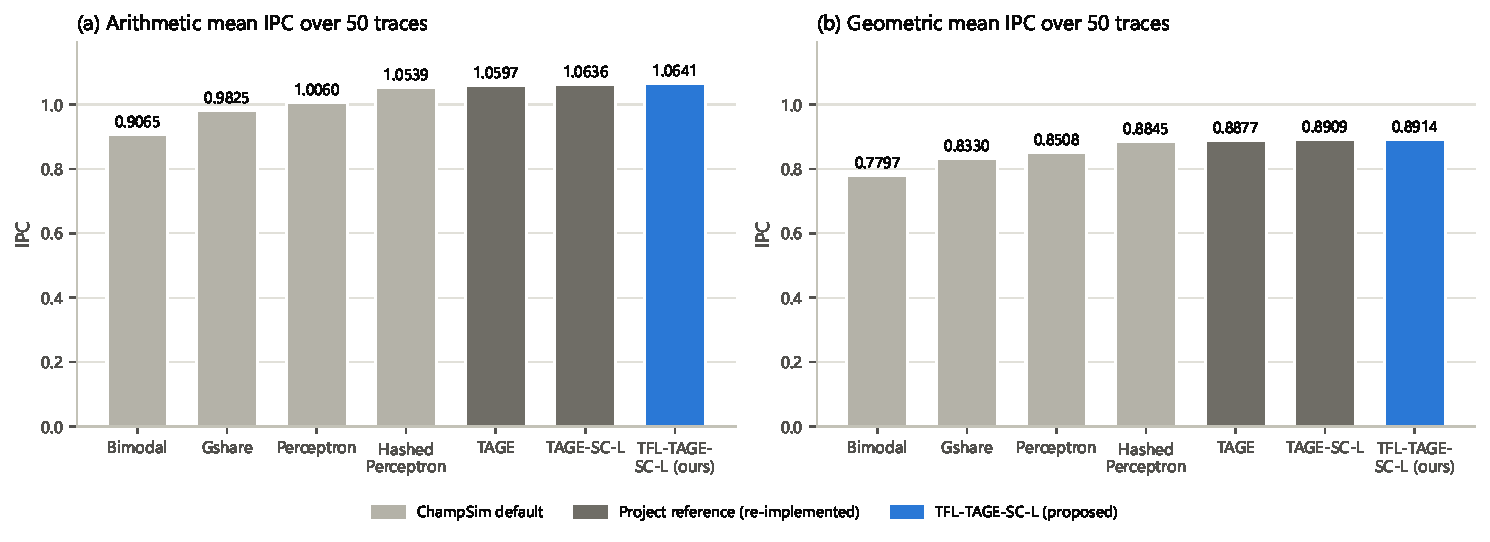
\includegraphics[width=\linewidth]{figures/fig1_ipc_comparison.pdf}
\caption{Arithmetic-mean (a) and geometric-mean (b) IPC of every predictor over \val{n_traces_agg} traces.}\label{fig:ipc}
\end{figure}

\begin{figure}[H]
\centering
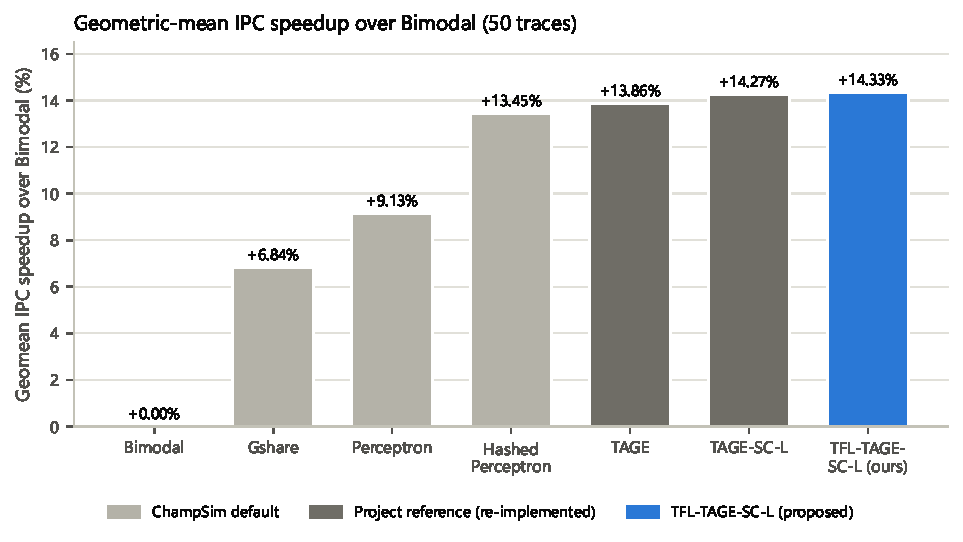
\includegraphics[width=0.7\linewidth]{figures/fig4_geomean_ipc_speedup.pdf}
\caption{Geometric-mean IPC speedup over bimodal.}\label{fig:speedup}
\end{figure}

\begin{figure}[H]
\centering
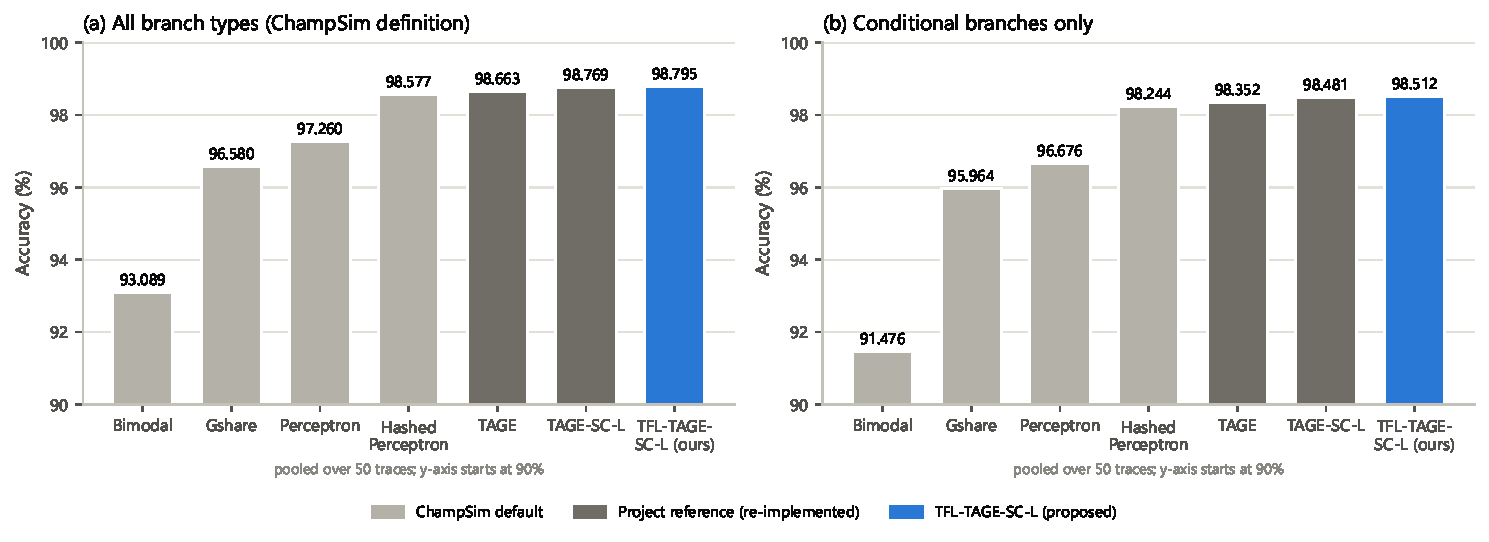
\includegraphics[width=\linewidth]{figures/fig2_accuracy_comparison.pdf}
\caption{Pooled branch prediction accuracy: all branch types (ChampSim's definition) and conditional branches only. The y-axis does not start at zero.}\label{fig:acc}
\end{figure}

\begin{figure}[H]
\centering
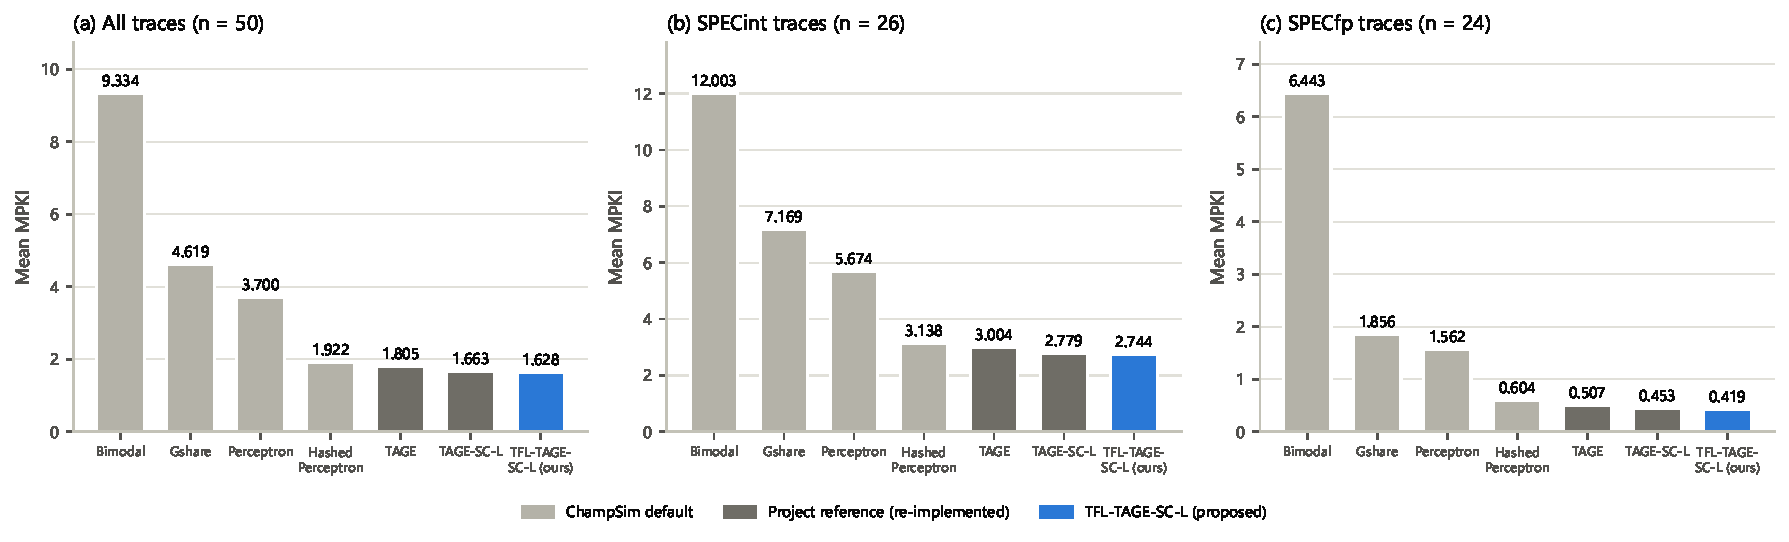
\includegraphics[width=\linewidth]{figures/fig3_mpki_comparison.pdf}
\caption{Mean MPKI over all traces, the SPECint traces and the SPECfp traces (note the different y-scales).}\label{fig:mpki}
\end{figure}

Table~\ref{tab:summary} and Figures~\ref{fig:ipc}--\ref{fig:mpki} summarise the \val{n_traces_agg} traces. \prop{} ranks first of the seven predictors on every aggregate: geometric-mean IPC (\val{prop_gm_ipc}), arithmetic-mean IPC (\val{prop_mean_ipc}), pooled accuracy over all branches (\val{prop_acc}\%) and over conditional branches (\val{prop_cacc}\%), and mean MPKI (\val{prop_mpki}).

The predictors form three clear tiers. The 4 KB ChampSim predictors are far behind: bimodal (\val{bim_mpki} MPKI), gshare (\val{gsh_mpki}) and perceptron (\val{perc_mpki}). The hashed perceptron (\val{hp_mpki}) is the best ChampSim predictor and is close to the TAGE family: TAGE (\val{tage_mpki}), TAGE-SC-L (\val{tsl_mpki}) and \prop{} (\val{prop_mpki}). Relative to bimodal, the geometric-mean speedup grows from \val{gsh_speedup_bim}\% (gshare) and \val{perc_speedup_bim}\% (perceptron) to \val{hp_speedup_bim}\% (hashed perceptron), \val{tage_speedup_bim}\% (TAGE), \val{tsl_speedup_bim}\% (TAGE-SC-L) and \val{prop_speedup_bim}\% (\prop{}) (Figure~\ref{fig:speedup}). Most of the available IPC gain is therefore obtained by any of the large predictors. The differences among the top four are an order of magnitude smaller than the gap to the 4 KB predictors.

The arithmetic and geometric means give the same ranking. The arithmetic means are higher because the per-trace IPCs span more than an order of magnitude: from about 2 (648.exchange2) to well below 0.5 on the memory-bound traces (605.mcf, 620.omnetpp, 623.xalancbmk, one 602.gcc window), whose IPC is limited by cache misses whatever the predictor (Appendix~\ref{app:all}). Accuracy differences look small in percentage points because most branches are easy; MPKI expresses the same difference in the units that matter for performance. The hashed perceptron's \val{hp_acc}\% and \prop{}'s \val{prop_acc}\% correspond to a \val{vs_hp_pct_mpki}\% difference in mean MPKI.

The per-predictor means hide a very uneven distribution over traces (Figure~\ref{fig:heatmap}). With \prop{}, \val{n_prop_mpki_below_0p1} traces have an MPKI below 0.1, and \val{n_prop_mpki_above_5} have an MPKI above 5. The five traces with the highest MPKI (\val{top5_mpki_traces}) account for \val{top5_mpki_share}\% of \prop{}'s mean MPKI; all are SPECint traces (mcf, leela, xz). Mean MPKI is therefore dominated by a few hard traces, a fact that matters when interpreting the comparisons below.


\subsection{\prop{} relative to each baseline}

\begin{table}[H]
\centering\small
\caption{\prop{} relative to each baseline over \val{n_traces_agg} traces (MPKI reductions from the means; IPC improvement from the geometric-mean speedup; per-trace counts by exact mispredictions and cycles).}\label{tab:comparison}
\resizebox{\linewidth}{!}{% generated by experiments/scripts/make_report_50trace.py -- do not edit
\begin{tabular}{lrrrrcc}
\toprule
Baseline & Baseline & MPKI & MPKI & Geomean IPC & Traces: lower / equal / & Traces: higher / equal / \\
 & mean MPKI & reduction & reduction (\%) & improvement (\%) & higher MPKI & lower IPC \\
\midrule
Bimodal & 9.334 & 7.7064 & 82.56 & +14.329 & 49 / 1 / 0 & 47 / 1 / 2 \\
Gshare & 4.619 & 2.9908 & 64.76 & +7.013 & 49 / 1 / 0 & 48 / 1 / 1 \\
Perceptron & 3.700 & 2.0727 & 56.01 & +4.767 & 49 / 1 / 0 & 48 / 1 / 1 \\
Hashed perceptron & 1.922 & 0.2939 & 15.29 & +0.772 & 46 / 2 / 2 & 45 / 2 / 3 \\
TAGE & 1.805 & 0.1773 & 9.82 & +0.413 & 46 / 3 / 1 & 46 / 3 / 1 \\
TAGE-SC-L & 1.663 & 0.0347 & 2.09 & +0.052 & 29 / 5 / 16 & 30 / 5 / 15 \\
\bottomrule
\end{tabular}
}
\end{table}

Table~\ref{tab:comparison} compares \prop{} with each baseline.

\paragraph{ChampSim's 4 KB predictors.} Against bimodal, gshare and perceptron, \prop{} reduces mean MPKI by \val{vs_bim_pct_mpki}\%, \val{vs_gsh_pct_mpki}\% and \val{vs_perc_pct_mpki}\%, and improves geometric-mean IPC by \val{vs_bim_ipc}\%, \val{vs_gsh_ipc}\% and \val{vs_perc_ipc}\%. It has fewer mispredictions on \val{vs_perc_mpki_win} of \val{n_traces} traces against each of them. The one remaining trace is a tie: on 649.fotonik3d\_s-1176B every predictor makes exactly the same number of mispredictions. These comparisons are not storage-equivalent (about 4 KB against 62 KB) and are included because these are the default predictors of the simulator.

\paragraph{Hashed perceptron (best ChampSim predictor, 64 KB).} This is the most relevant comparison with a ChampSim predictor, because its storage is similar and slightly larger. \prop{} reduces mean MPKI from \val{hp_mpki} to \val{prop_mpki} (\val{vs_hp_pct_mpki}\%) and improves geometric-mean IPC by \val{vs_hp_ipc}\% (arithmetic mean \val{vs_hp_meanipc}\%). The gain is broad rather than driven by a few traces:
\begin{itemize}
\item \prop{} has fewer mispredictions on \val{vs_hp_mpki_win} traces and more on \val{vs_hp_mpki_loss} (\val{vs_hp_mpki_tie} ties).
\item It has higher IPC on \val{vs_hp_ipc_win} traces and lower IPC on \val{vs_hp_ipc_loss}. No IPC loss exceeds 0.1\%: the largest is \val{vs_hp_worst_pct}\% on \val{vs_hp_worst_trace}.
\item \val{vs_hp_n_ipc_gt0p1} traces gain more than 0.1\% IPC, and the median per-trace IPC change is \val{vs_hp_median_ipc}\%.
\item The largest single contributor (\val{vs_hp_top_trace}) provides only \val{vs_hp_top_share}\% of the MPKI reduction; without it the reduction is still \val{vs_hp_pct_mpki_excl_top}\%.
\end{itemize}

\paragraph{TAGE.} Against our TAGE with the same tagged tables but no corrector or loop predictor, \prop{} reduces mean MPKI by \val{vs_tage_pct_mpki}\% and improves geometric-mean IPC by \val{vs_tage_ipc}\%. It has fewer mispredictions on \val{vs_tage_mpki_win} traces and more on \val{vs_tage_mpki_loss}. This difference combines the statistical corrector, the loop predictor and the loop-structure components.

\paragraph{TAGE-SC-L (the same predictor without the contribution).} This comparison isolates the effect of the proposed loop-structure components and the target-free inference. The effect is positive but small:
\begin{itemize}
\item Mean MPKI falls from \val{tsl_mpki} to \val{prop_mpki} (\val{vs_tsl_pct_mpki}\%). Pooled accuracy rises by \val{vs_tsl_acc_pp} percentage points, and geometric-mean IPC by \val{vs_tsl_ipc}\%.
\item \prop{} has fewer mispredictions on \val{vs_tsl_mpki_win} traces, more on \val{vs_tsl_mpki_loss} and the same number on \val{vs_tsl_mpki_tie}.
\item For IPC the count is \val{vs_tsl_ipc_win} higher, \val{vs_tsl_ipc_loss} lower and \val{vs_tsl_ipc_tie} equal.
\end{itemize}
The losses are all tiny: the largest MPKI increase on any trace is \val{vs_tsl_worstm} (\val{vs_tsl_worstm_trace}), and the largest IPC loss is \val{vs_tsl_worst_pct}\% (\val{vs_tsl_worst_trace}). The gains, in contrast, are concentrated:
\begin{itemize}
\item On 627.cam4\_s-490B MPKI falls by \val{vs_tsl_bestm} and IPC rises by \val{vs_tsl_best_pct}\%. This one trace provides \val{vs_tsl_top_share}\% of the mean-MPKI reduction; without it, the reduction over the other 49 traces is \val{vs_tsl_pct_mpki_excl_top}\%.
\item On \val{vs_tsl_n_ipc_flat} traces the IPC changes by less than 0.01\% in either direction, and the median per-trace IPC change is \val{vs_tsl_median_ipc}\%.
\end{itemize}
The improvement over TAGE-SC-L is therefore consistent in sign but modest in size on most workloads, and larger on a few.


\subsection{Per-trace analysis}\label{sec:pertrace}

\begin{figure}[H]
\centering
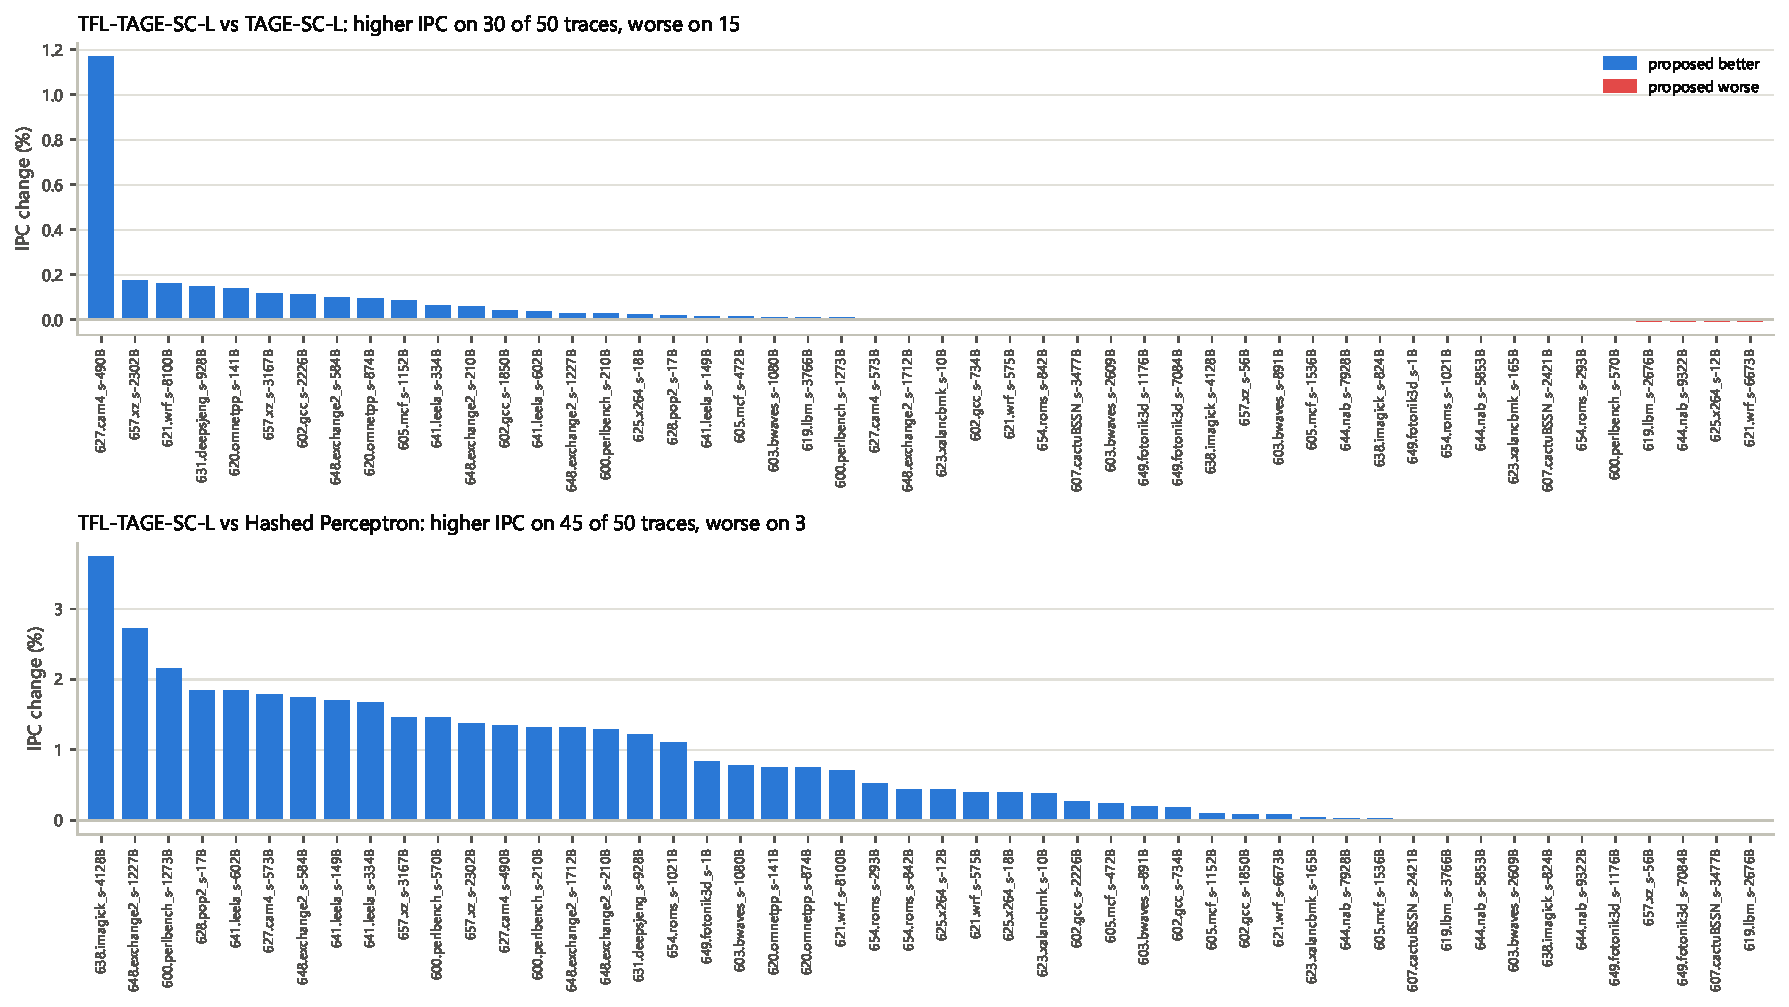
\includegraphics[width=\linewidth]{figures/fig5_per_trace_ipc_vs_best_baselines.pdf}
\caption{Per-trace IPC change of \prop{} relative to the best baseline by geometric-mean IPC and the best ChampSim default predictor, sorted.}\label{fig:pertrace_ipc}
\end{figure}

\begin{figure}[H]
\centering
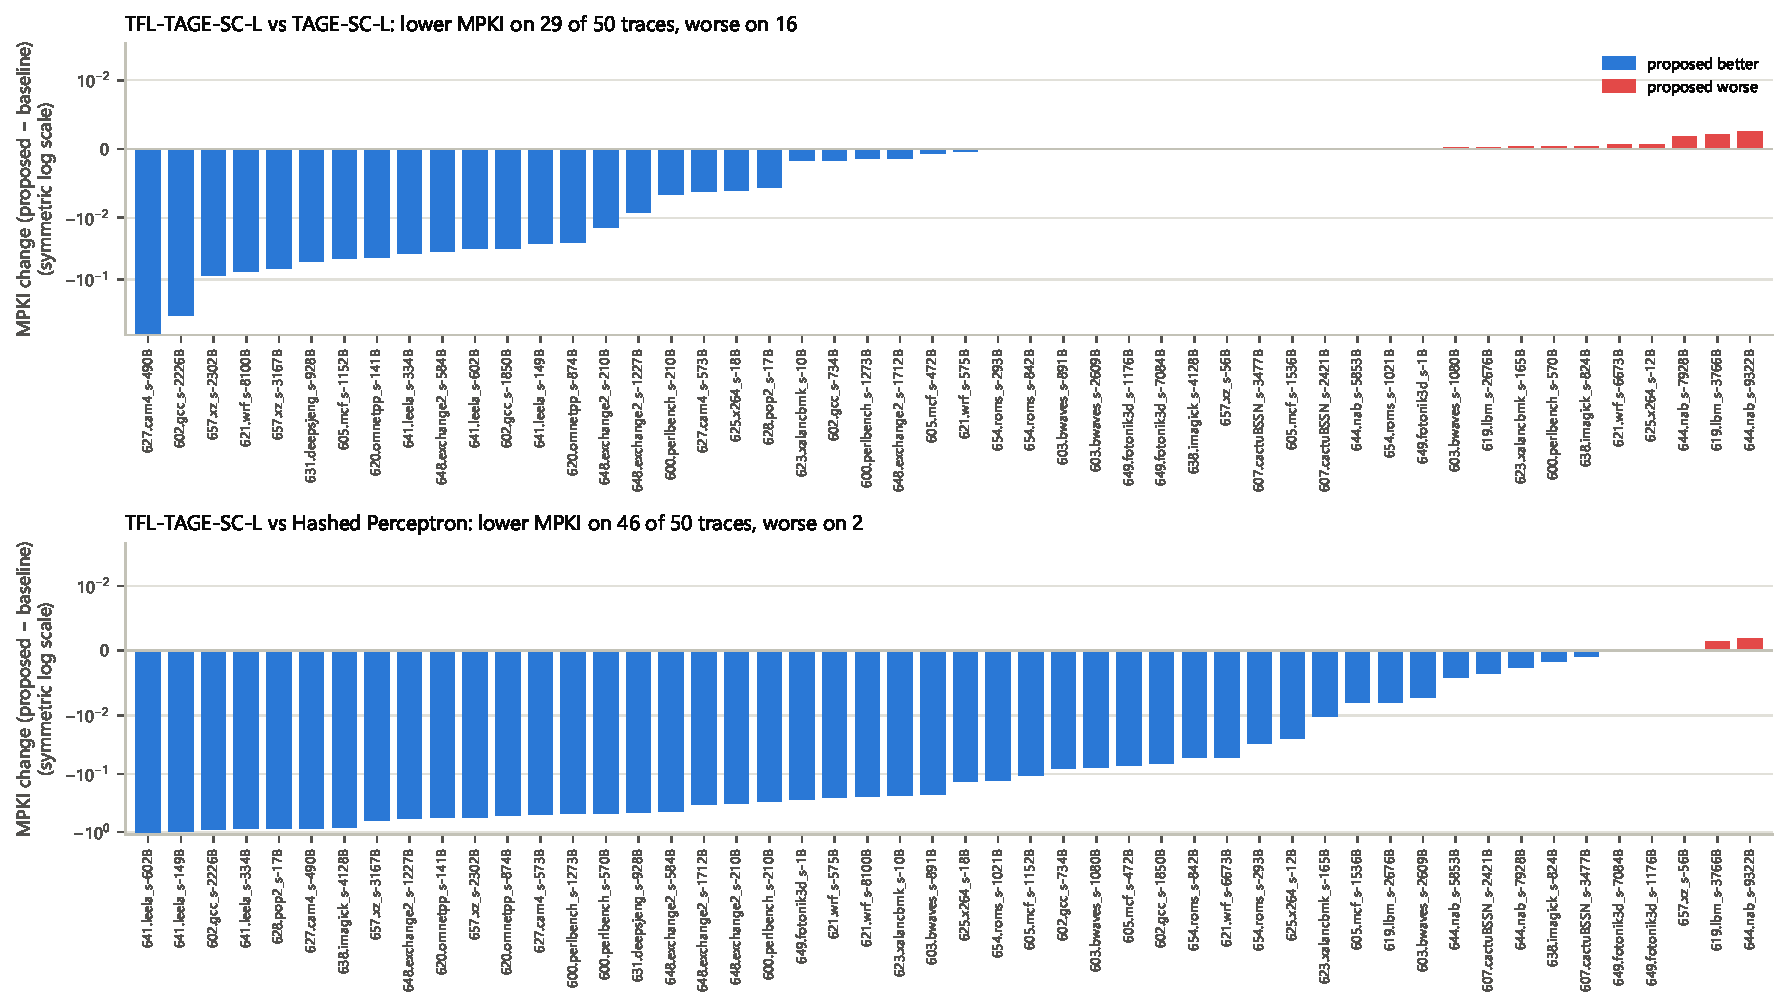
\includegraphics[width=\linewidth]{figures/fig6_per_trace_mpki_change.pdf}
\caption{Per-trace MPKI change of \prop{} (negative = fewer mispredictions; symmetric-log scale, linear within $\pm 0.01$).}\label{fig:pertrace_mpki}
\end{figure}

\begin{table}[H]
\centering\small
\caption{Traces with the largest IPC gains and losses of \prop{} relative to the best baseline and the best ChampSim default ($\Delta$MPKI = proposed $-$ baseline).}\label{tab:extremes}
\resizebox{\linewidth}{!}{% generated by experiments/scripts/make_report_50trace.py -- do not edit
\begin{tabular}{llrrlrr}
\toprule
 & \multicolumn{3}{c}{Largest IPC gains} & \multicolumn{3}{c}{Lowest IPC changes (losses, if any)} \\
\cmidrule(lr){2-4}\cmidrule(lr){5-7}
Baseline & Trace & $\Delta$IPC (\%) & $\Delta$MPKI & Trace & $\Delta$IPC (\%) & $\Delta$MPKI \\
\midrule
TAGE-SC-L & 627.cam4\_s-490B & +1.171 & -0.7499 & 621.wrf\_s-6673B & -0.009 & +0.0007 \\
 & 657.xz\_s-2302B & +0.176 & -0.0869 & 625.x264\_s-12B & -0.009 & +0.0007 \\
 & 621.wrf\_s-8100B & +0.160 & -0.0750 & 644.nab\_s-9322B & -0.008 & +0.0026 \\
 & 631.deepsjeng\_s-928B & +0.148 & -0.0520 & 619.lbm\_s-2676B & -0.006 & +0.0003 \\
 & 620.omnetpp\_s-141B & +0.138 & -0.0438 & 600.perlbench\_s-570B & -0.002 & +0.0004 \\
 & 657.xz\_s-3167B & +0.115 & -0.0656 & 654.roms\_s-293B & -0.001 & -0.0000 \\
\midrule
Hashed perceptron & 638.imagick\_s-4128B & +3.750 & -0.8418 & 619.lbm\_s-2676B & -0.018 & -0.0080 \\
 & 648.exchange2\_s-1227B & +2.729 & -0.5905 & 607.cactuBSSN\_s-3477B & -0.009 & -0.0009 \\
 & 600.perlbench\_s-1273B & +2.158 & -0.4864 & 649.fotonik3d\_s-7084B & -0.000 & -0.0000 \\
 & 628.pop2\_s-17B & +1.845 & -0.8691 & 657.xz\_s-56B & +0.000 & +0.0000 \\
 & 641.leela\_s-602B & +1.845 & -1.0569 & 649.fotonik3d\_s-1176B & +0.000 & +0.0000 \\
 & 627.cam4\_s-573B & +1.791 & -0.5023 & 644.nab\_s-9322B & +0.000 & +0.0019 \\
\bottomrule
\end{tabular}
}
\end{table}

Figures~\ref{fig:pertrace_ipc} and~\ref{fig:pertrace_mpki} show the per-trace changes relative to TAGE-SC-L (the best baseline by geometric-mean IPC) and the hashed perceptron (the best ChampSim predictor). Table~\ref{tab:extremes} lists the extremes, and Table~\ref{tab:traces} lists every trace.

\paragraph{Best predictor per trace.} \prop{} has the fewest mispredictions on \val{n_best_mpki_prop} of the \val{n_traces} traces: alone on \val{n_sole_mpki_prop}, and tied with others on the rest. TAGE-SC-L is best or tied on \val{n_best_mpki_tsl} (alone on \val{n_sole_mpki_tsl}), and no other predictor is the sole best on any trace. On \val{n_tied_best_mpki} traces several predictors make exactly the same, minimal number of mispredictions. On 649.fotonik3d\_s-1176B all seven do; on 657.xz\_s-56B the four large predictors make none at all.

By cycles, \prop{} is fastest or tied on \val{n_best_ipc_prop} traces and TAGE-SC-L on \val{n_best_ipc_tsl}. The hashed perceptron is fastest alone on \val{n_sole_ipc_hp} traces and TAGE on \val{n_sole_ipc_tage}. These are traces with almost no mispredictions, where cycle counts differ by a few hundredths of a percent for reasons unrelated to prediction quality. For example, on 649.fotonik3d\_s-7084B the hashed perceptron is fastest although it mispredicts more than the TAGE family.

\paragraph{Where the gains come from.} Against the hashed perceptron, the largest IPC gains are on \val{vs_hp_best_trace} (\val{vs_hp_best_pct}\%), 648.exchange2, 600.perlbench, 628.pop2 and 641.leela (Table~\ref{tab:extremes}). On these traces every TAGE-family predictor is clearly more accurate than the hashed perceptron, which suggests branch patterns that tagged long-history tables capture better than a hashed perceptron. On 638.imagick\_s-4128B, for instance, TAGE-SC-L and \prop{} make almost no mispredictions, while the hashed perceptron does not reach that level (Figure~\ref{fig:heatmap}).

Our TAGE alone has more mispredictions than the hashed perceptron on \val{n_tage_worse_hp} traces. With the statistical corrector and loop predictor (TAGE-SC-L) that number falls to \val{n_tsl_worse_hp}. For \prop{} it is \val{n_prop_worse_hp}, both by at most \val{vs_hp_worstm} MPKI. The corrector is thus what makes the TAGE family robust on traces where a perceptron-style predictor does well.

\paragraph{Effect of the loop-structure components.} Relative to TAGE-SC-L, the largest reductions are on:
\begin{itemize}
\item 627.cam4\_s-490B (MPKI \val{vs_tsl_bestm} lower);
\item 602.gcc\_s-2226B, both 657.xz traces, 621.wrf\_s-8100B, 631.deepsjeng, 605.mcf\_s-1152B and 620.omnetpp\_s-141B.
\end{itemize}
In relative terms the largest reductions are on 602.gcc. On \val{tsl_rel1_trace} MPKI falls from \val{tsl_rel1_from} to \val{tsl_rel1_to} (\val{tsl_rel1_pct}\%), and on \val{tsl_rel2_trace} from \val{tsl_rel2_from} to \val{tsl_rel2_to} (\val{tsl_rel2_pct}\%). However, the median relative change over the \val{tsl_rel_n} traces on which TAGE-SC-L has an MPKI of at least 0.05 is only \val{tsl_rel_median_pct}\%.

The \val{vs_tsl_mpki_loss} traces with more mispredictions than TAGE-SC-L belong to twelve benchmarks (the largest increases: 644.nab, 619.lbm, 625.x264, 621.wrf). Every increase is at most \val{vs_tsl_worstm} MPKI: at most a few hundred extra mispredictions in 200M instructions, and fewer than 100 on most of these traces. These look like the expected side effect of adding inputs to the corrector (more aliasing and slower training), not a systematic failure on a workload class.

\paragraph{Hard traces.} All predictors struggle on the same traces: 605.mcf\_s-1152B, the three 641.leela traces, 657.xz\_s-2302B, 631.deepsjeng and 620.omnetpp (Figure~\ref{fig:heatmap}). There even \prop{} mispredicts several times per thousand instructions, and it removes at most about 1.5\% of TAGE-SC-L's mispredictions. These programs (game-tree search, network simulation, graph optimisation, compression) are known for branches that depend on data values rather than on branch history. None of the evaluated predictors, including the proposed one, addresses that kind of branch.


{\small\setlength{\tabcolsep}{4pt}% generated by experiments/scripts/make_report_50trace.py -- do not edit
\begin{longtable}{llrrrrrrr}
\caption{Per-trace characteristics and results (measured window). Br/KI = branches per 1,000 instructions; $\Delta$IPC relative to TAGE-SC-L and the hashed perceptron.}\label{tab:traces}\\
\toprule
Trace & Set & Br/KI & Cond. & MPKI & MPKI & MPKI & $\Delta$IPC (\%) & $\Delta$IPC (\%) \\
 & & & share & HP & TSL & proposed & vs TSL & vs HP \\
\midrule
\endhead
600.perlbench\_s-1273B & add/INT & 140.1 & 70\% & 1.120 & 0.635 & 0.634 & +0.008 & +2.158 \\
600.perlbench\_s-210B & add/INT & 140.1 & 71\% & 0.954 & 0.666 & 0.659 & +0.025 & +1.323 \\
600.perlbench\_s-570B & add/INT & 164.9 & 72\% & 1.534 & 1.051 & 1.051 & -0.002 & +1.454 \\
602.gcc\_s-1850B & orig/INT & 256.4 & 83\% & 0.097 & 0.063 & 0.032 & +0.039 & +0.084 \\
602.gcc\_s-2226B & add/INT & 356.4 & 98\% & 1.057 & 0.534 & 0.149 & +0.114 & +0.263 \\
602.gcc\_s-734B & add/INT & 240.2 & 80\% & 0.235 & 0.155 & 0.153 & +0.003 & +0.179 \\
603.bwaves\_s-1080B & add/FP & 145.3 & 90\% & 0.094 & 0.014 & 0.015 & +0.010 & +0.771 \\
603.bwaves\_s-2609B & add/FP & 25.0 & 100\% & 0.007 & 0.000 & 0.000 & +0.000 & +0.007 \\
603.bwaves\_s-891B & add/FP & 167.6 & 96\% & 0.223 & 0.000 & 0.000 & -0.000 & +0.190 \\
605.mcf\_s-1152B & orig/INT & 258.4 & 74\% & 13.981 & 13.920 & 13.874 & +0.087 & +0.089 \\
605.mcf\_s-1536B & add/INT & 155.8 & 57\% & 0.019 & 0.011 & 0.011 & -0.000 & +0.020 \\
605.mcf\_s-472B & add/INT & 128.9 & 92\% & 1.106 & 1.033 & 1.033 & +0.013 & +0.240 \\
607.cactuBSSN\_s-2421B & orig/FP & 1.4 & 52\% & 0.007 & 0.003 & 0.003 & -0.001 & +0.016 \\
607.cactuBSSN\_s-3477B & add/FP & 8.9 & 61\% & 0.001 & 0.000 & 0.000 & +0.000 & -0.009 \\
619.lbm\_s-2676B & orig/FP & 12.1 & 95\% & 0.109 & 0.101 & 0.101 & -0.006 & -0.018 \\
619.lbm\_s-3766B & add/FP & 15.6 & 87\% & 0.366 & 0.365 & 0.367 & +0.010 & +0.013 \\
620.omnetpp\_s-141B & orig/INT & 209.9 & 64\% & 3.838 & 3.322 & 3.278 & +0.138 & +0.749 \\
620.omnetpp\_s-874B & add/INT & 208.0 & 64\% & 3.727 & 3.237 & 3.211 & +0.095 & +0.744 \\
621.wrf\_s-575B & add/FP & 134.0 & 77\% & 0.475 & 0.224 & 0.223 & +0.002 & +0.398 \\
621.wrf\_s-6673B & add/FP & 60.1 & 93\% & 0.079 & 0.026 & 0.027 & -0.009 & +0.083 \\
621.wrf\_s-8100B & add/FP & 123.4 & 81\% & 1.166 & 0.993 & 0.918 & +0.160 & +0.713 \\
623.xalancbmk\_s-10B & orig/INT & 258.7 & 90\% & 0.692 & 0.455 & 0.453 & +0.005 & +0.387 \\
623.xalancbmk\_s-165B & add/INT & 277.6 & 95\% & 0.031 & 0.020 & 0.020 & -0.001 & +0.032 \\
625.x264\_s-12B & orig/INT & 42.4 & 84\% & 0.079 & 0.053 & 0.054 & -0.009 & +0.431 \\
625.x264\_s-18B & add/INT & 47.0 & 84\% & 0.662 & 0.533 & 0.527 & +0.023 & +0.391 \\
627.cam4\_s-490B & add/FP & 96.0 & 95\% & 4.696 & 4.578 & 3.828 & +1.171 & +1.351 \\
627.cam4\_s-573B & add/FP & 133.5 & 86\% & 0.980 & 0.484 & 0.478 & +0.007 & +1.791 \\
628.pop2\_s-17B & add/FP & 152.5 & 93\% & 1.197 & 0.333 & 0.328 & +0.018 & +1.845 \\
631.deepsjeng\_s-928B & orig/INT & 147.1 & 66\% & 4.166 & 3.761 & 3.709 & +0.148 & +1.221 \\
638.imagick\_s-4128B & add/FP & 193.5 & 98\% & 0.842 & 0.000 & 0.000 & +0.000 & +3.750 \\
638.imagick\_s-824B & orig/FP & 161.3 & 64\% & 0.090 & 0.088 & 0.089 & -0.000 & +0.003 \\
641.leela\_s-149B & add/INT & 165.5 & 62\% & 10.929 & 9.962 & 9.936 & +0.016 & +1.703 \\
641.leela\_s-334B & add/INT & 173.8 & 63\% & 8.304 & 7.463 & 7.425 & +0.062 & +1.670 \\
641.leela\_s-602B & add/INT & 170.2 & 63\% & 10.043 & 9.018 & 8.986 & +0.034 & +1.845 \\
644.nab\_s-5853B & add/FP & 96.8 & 69\% & 0.015 & 0.011 & 0.011 & -0.001 & +0.007 \\
644.nab\_s-7928B & add/FP & 96.0 & 83\% & 1.488 & 1.484 & 1.486 & -0.000 & +0.021 \\
644.nab\_s-9322B & add/FP & 128.8 & 81\% & 2.118 & 2.117 & 2.120 & -0.008 & +0.000 \\
648.exchange2\_s-1227B & add/INT & 142.8 & 91\% & 1.372 & 0.791 & 0.782 & +0.029 & +2.729 \\
648.exchange2\_s-1712B & add/INT & 134.1 & 92\% & 0.721 & 0.391 & 0.389 & +0.005 & +1.321 \\
648.exchange2\_s-210B & add/INT & 136.2 & 92\% & 0.822 & 0.520 & 0.506 & +0.057 & +1.289 \\
648.exchange2\_s-584B & add/INT & 140.7 & 90\% & 1.228 & 0.823 & 0.787 & +0.100 & +1.741 \\
649.fotonik3d\_s-1176B & add/FP & 17.6 & 100\% & 0.004 & 0.004 & 0.004 & +0.000 & +0.000 \\
649.fotonik3d\_s-1B & add/FP & 237.8 & 66\% & 0.277 & 0.001 & 0.001 & -0.000 & +0.840 \\
649.fotonik3d\_s-7084B & add/FP & 6.9 & 100\% & 0.000 & 0.000 & 0.000 & +0.000 & -0.000 \\
654.roms\_s-1021B & add/FP & 150.1 & 83\% & 0.130 & 0.001 & 0.001 & -0.001 & +1.110 \\
654.roms\_s-293B & add/FP & 35.5 & 100\% & 0.032 & 0.001 & 0.001 & -0.001 & +0.525 \\
654.roms\_s-842B & add/FP & 164.4 & 81\% & 0.105 & 0.052 & 0.052 & +0.001 & +0.438 \\
657.xz\_s-2302B & orig/INT & 125.0 & 85\% & 9.417 & 8.950 & 8.863 & +0.176 & +1.381 \\
657.xz\_s-3167B & add/INT & 148.4 & 93\% & 5.445 & 4.878 & 4.813 & +0.115 & +1.465 \\
657.xz\_s-56B & add/INT & 20.1 & 97\% & 0.000 & 0.000 & 0.000 & +0.000 & +0.000 \\
\bottomrule
\end{longtable}
}

\begin{figure}[p]
\centering
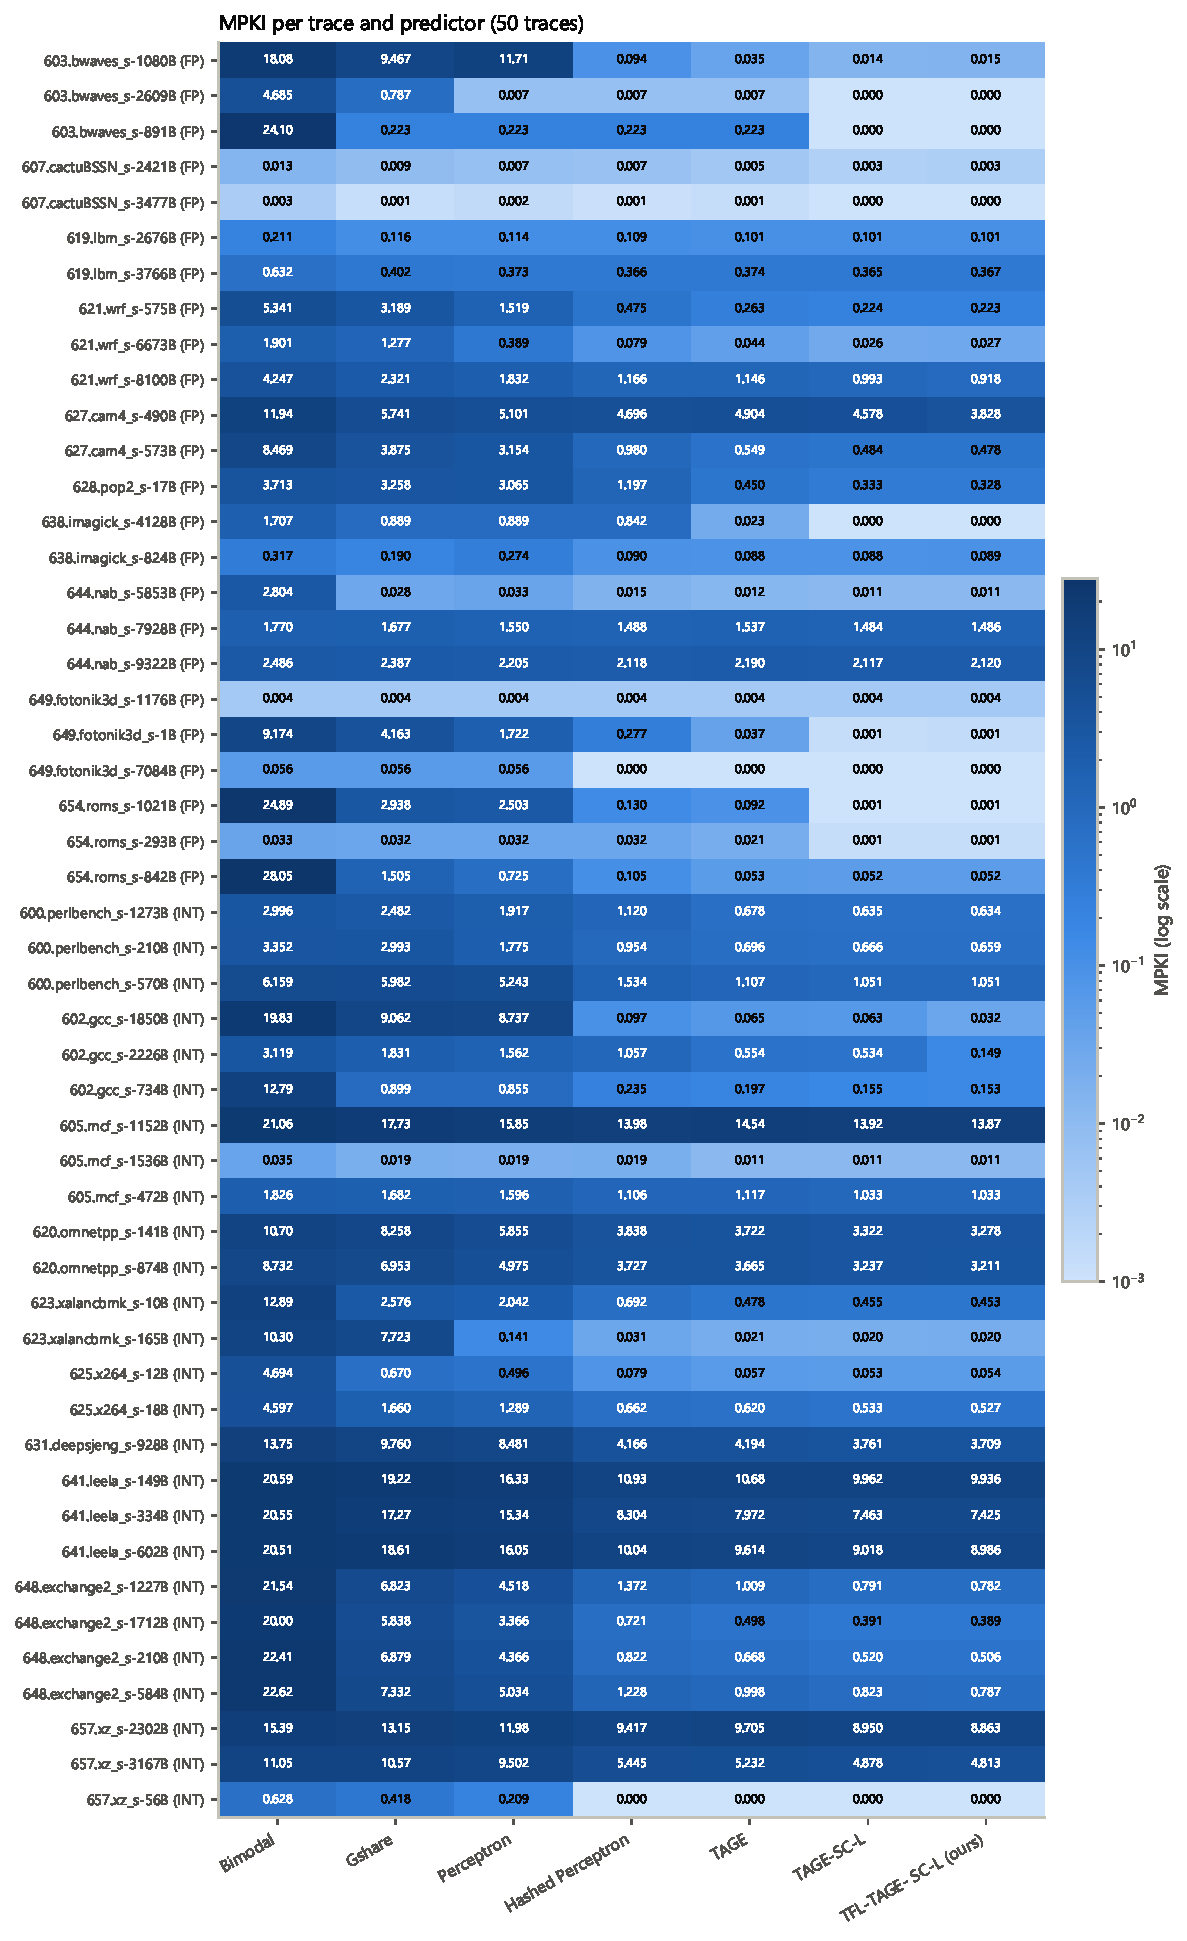
\includegraphics[height=0.9\textheight]{figures/fig7_mpki_heatmap.pdf}
\caption{MPKI of every predictor on every trace (log colour scale), grouped into SPECfp and SPECint.}\label{fig:heatmap}
\end{figure}

\subsection{Generalisation: original 10 versus additional 40 traces}\label{sec:generalisation}

\begin{table}[H]
\centering\small
\caption{Mean MPKI and the gain of \prop{} on trace subsets (HP = hashed perceptron, TSL = TAGE-SC-L; IPC as geometric-mean improvement).}\label{tab:subsets}
\resizebox{\linewidth}{!}{% generated by experiments/scripts/make_report_50trace.py -- do not edit
\begin{tabular}{lrrrrrrr}
\toprule
Subset & $n$ & \multicolumn{3}{c}{Mean MPKI} & \multicolumn{3}{c}{Proposed vs.\ baseline} \\
\cmidrule(lr){3-5}\cmidrule(lr){6-8}
 & & Hashed perc. & TAGE-SC-L & Proposed & MPKI red.\ vs HP & MPKI red.\ vs TSL & IPC vs TSL \\
\midrule
All traces & 50 & 1.922 & 1.663 & 1.628 & 15.29\% & 2.09\% & +0.052\% \\
Original 10 & 10 & 3.247 & 3.072 & 3.046 & 6.22\% & 0.85\% & +0.058\% \\
Additional 40 & 40 & 1.590 & 1.310 & 1.273 & 19.93\% & 2.82\% & +0.051\% \\
SPECint & 26 & 3.138 & 2.779 & 2.744 & 12.56\% & 1.26\% & +0.049\% \\
SPECfp & 24 & 0.604 & 0.453 & 0.419 & 30.68\% & 7.61\% & +0.056\% \\
\bottomrule
\end{tabular}
}
\end{table}

\begin{figure}[H]
\centering
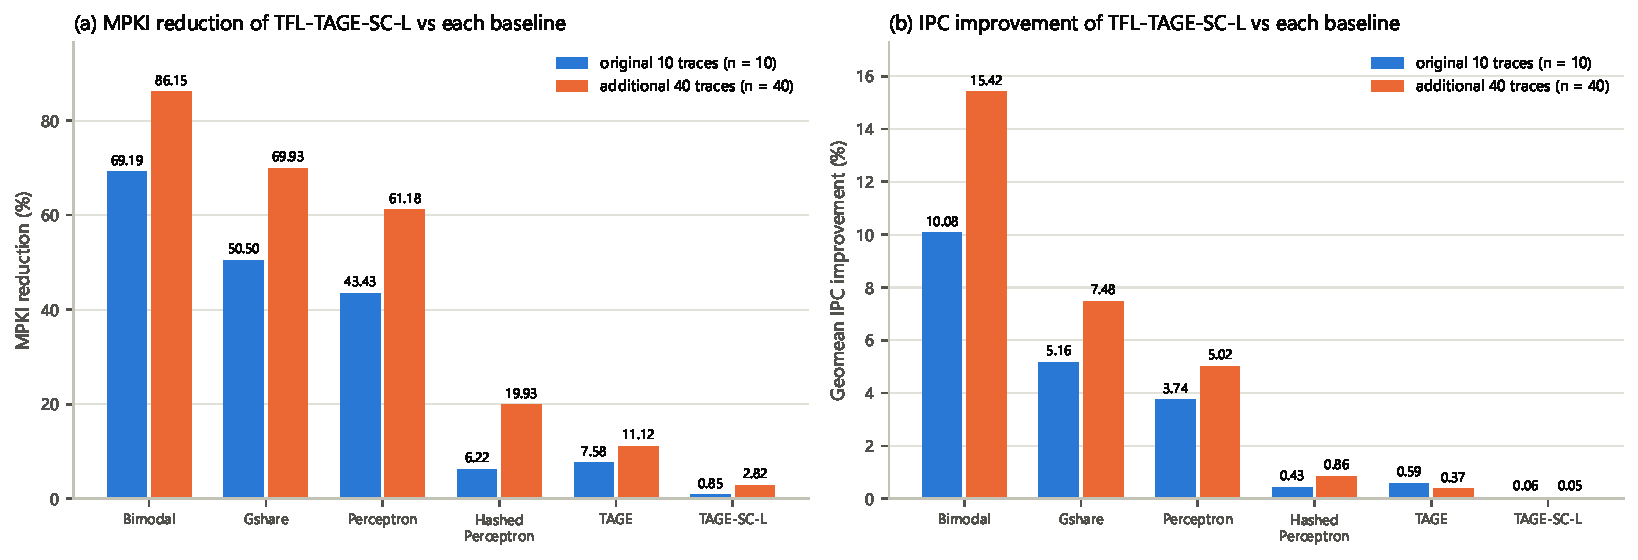
\includegraphics[width=\linewidth]{figures/fig10_generalisation_original_vs_additional.pdf}
\caption{MPKI reduction and geometric-mean IPC improvement of \prop{} relative to each baseline, on the original 10 traces and on the 40 additional traces.}\label{fig:generalisation}
\end{figure}

The design was developed on the original ten programs. Tuning used a different instruction window, but the final configuration was also checked on the reported window. The \val{n_add} additional traces were never used for design or tuning, which makes them the cleaner test (Table~\ref{tab:subsets}, Figure~\ref{fig:generalisation}).

\paragraph{The result carries over.} On the original ten traces \prop{} reduces mean MPKI by \val{original10_hp_red}\% relative to the hashed perceptron and by \val{original10_tsl_red}\% relative to TAGE-SC-L, with geometric-mean IPC gains of \val{original10_hp_ipcimp}\% and \val{original10_tsl_ipcimp}\%. These are exactly the values of the earlier study. On the \val{n_add} additional traces the corresponding values are:
\begin{itemize}
\item relative to the hashed perceptron: \val{additional40_hp_red}\% lower MPKI and \val{additional40_hp_ipcimp}\% higher geometric-mean IPC;
\item relative to TAGE-SC-L: \val{additional40_tsl_red}\% lower MPKI and \val{additional40_tsl_ipcimp}\% higher geometric-mean IPC.
\end{itemize}
\prop{} has the lowest mean MPKI and the highest geometric-mean IPC in both subsets, so its first place does not depend on the traces used during design. The order among the baselines does change: TAGE is behind the hashed perceptron on the original ten but ahead on the additional traces (below).

\paragraph{Why the relative MPKI gain is larger on the additional traces.} Two effects explain why the percentage reductions are larger on the new traces, while the IPC improvement over TAGE-SC-L is about the same in both subsets.
\begin{itemize}
\item The additional set contains many SPECfp traces with low MPKI (mean MPKI of the hashed perceptron \val{additional40_hp_mpki} against \val{original10_hp_mpki} on the original ten). A small absolute reduction is therefore a larger percentage.
\item It contains 627.cam4\_s-490B, the trace with the largest gain over TAGE-SC-L.
\end{itemize}
The original ten traces are dominated by hard SPECint traces (605.mcf, 657.xz, 631.deepsjeng, 620.omnetpp). There, even our TAGE is slightly worse than the hashed perceptron (\val{original10_tage_mpki} against \val{original10_hp_mpki} MPKI); on the additional traces TAGE is clearly better (\val{additional40_tage_mpki} against \val{additional40_hp_mpki}). The earlier study's conclusion that a TAGE of comparable size does not beat the hashed perceptron on average was thus a property of its ten traces and does not hold on the larger set.

\paragraph{SPECint and SPECfp.} \prop{} reduces mean MPKI relative to TAGE-SC-L by \val{INT_tsl_red}\% on the \val{INT_n} SPECint traces and by \val{FP_tsl_red}\% on the \val{FP_n} SPECfp traces. Relative to the hashed perceptron the reductions are \val{INT_hp_red}\% and \val{FP_hp_red}\%. The geometric-mean IPC gain over TAGE-SC-L is similar in both suites (\val{INT_tsl_ipcimp}\% and \val{FP_tsl_ipcimp}\%). The gain over the hashed perceptron is larger on SPECint (\val{INT_hp_ipcimp}\% against \val{FP_hp_ipcimp}\%), where the absolute number of mispredictions removed is larger.

The overlap between the two subsets must be kept in mind: 12 of the 40 additional traces are further SimPoints of benchmarks that also appear among the original ten (for example 602.gcc, 605.mcf, 657.xz). They are different program phases, but not different programs. The other 28 come from ten benchmarks that the earlier study did not use at all.


\subsection{Storage versus performance}

\begin{figure}[H]
\centering
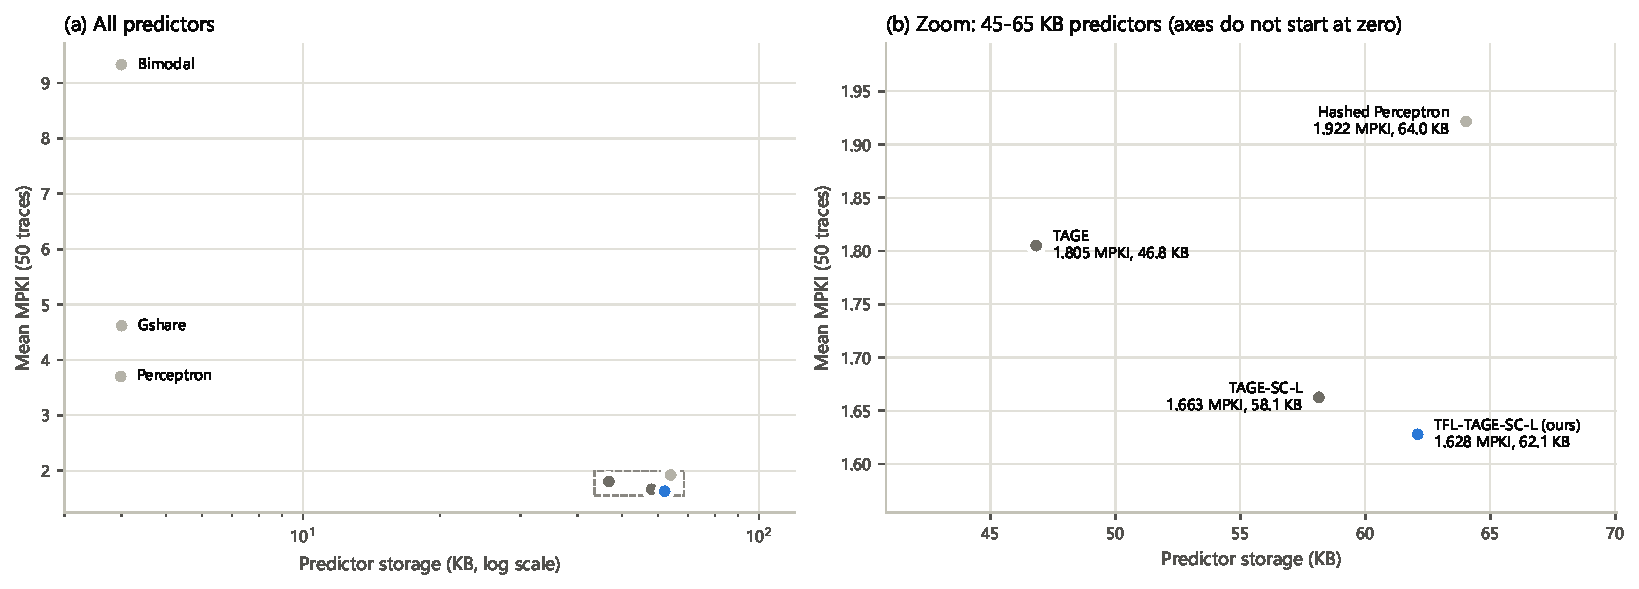
\includegraphics[width=\linewidth]{figures/fig8_storage_vs_mpki.pdf}
\caption{Storage against mean MPKI; (b) zooms on the 45--65 KB predictors.}\label{fig:storage}
\end{figure}

Figure~\ref{fig:storage} places every predictor by storage and mean MPKI.

\paragraph{The three storage classes.}
\begin{itemize}
\item \textbf{About 4 KB.} The perceptron is the most accurate (\val{perc_mpki} MPKI at \val{perc_kb} KB). It dominates gshare and bimodal, which use the same or slightly more storage.
\item \textbf{47--64 KB.} The hashed perceptron is dominated by both TAGE (smaller and more accurate) and \prop{} (\val{hp_minus_prop_bits} bits smaller, \val{vs_hp_pct_mpki}\% lower MPKI).
\end{itemize}
Among the predictors evaluated, the best accuracy for a given storage is therefore obtained by the perceptron at about 4 KB, and above that by TAGE (\val{tage_kb} KB), TAGE-SC-L (\val{tsl_kb} KB) and \prop{} (\val{prop_kb} KB).

\paragraph{Diminishing returns along the TAGE family.} Going from TAGE to TAGE-SC-L adds \val{tsl_kb} $-$ \val{tage_kb} KB (corrector and loop predictor) and lowers mean MPKI from \val{tage_mpki} to \val{tsl_mpki}. Going from TAGE-SC-L to \prop{} adds \val{prop_minus_tsl_kb} KB (\val{prop_minus_tsl_pct}\%) and lowers it to \val{prop_mpki} (\val{vs_tsl_pct_mpki}\%). Per kilobyte, the loop-structure components are thus less effective than the corrector, which is consistent with their effect being concentrated on a few traces.

\paragraph{The equal-storage question.} The experiment does not show whether spending the same \val{prop_minus_tsl_kb} KB on larger TAGE-SC-L tables would give a similar gain: no storage-matched TAGE-SC-L was evaluated, neither here nor in the earlier study. Given the diminishing returns above and the small size of the gain, this is the main open question about the contribution. The comparison with the hashed perceptron, which is larger than \prop{}, is not affected by this caveat.


\subsection{MPKI reduction versus IPC gain}

\begin{figure}[H]
\centering
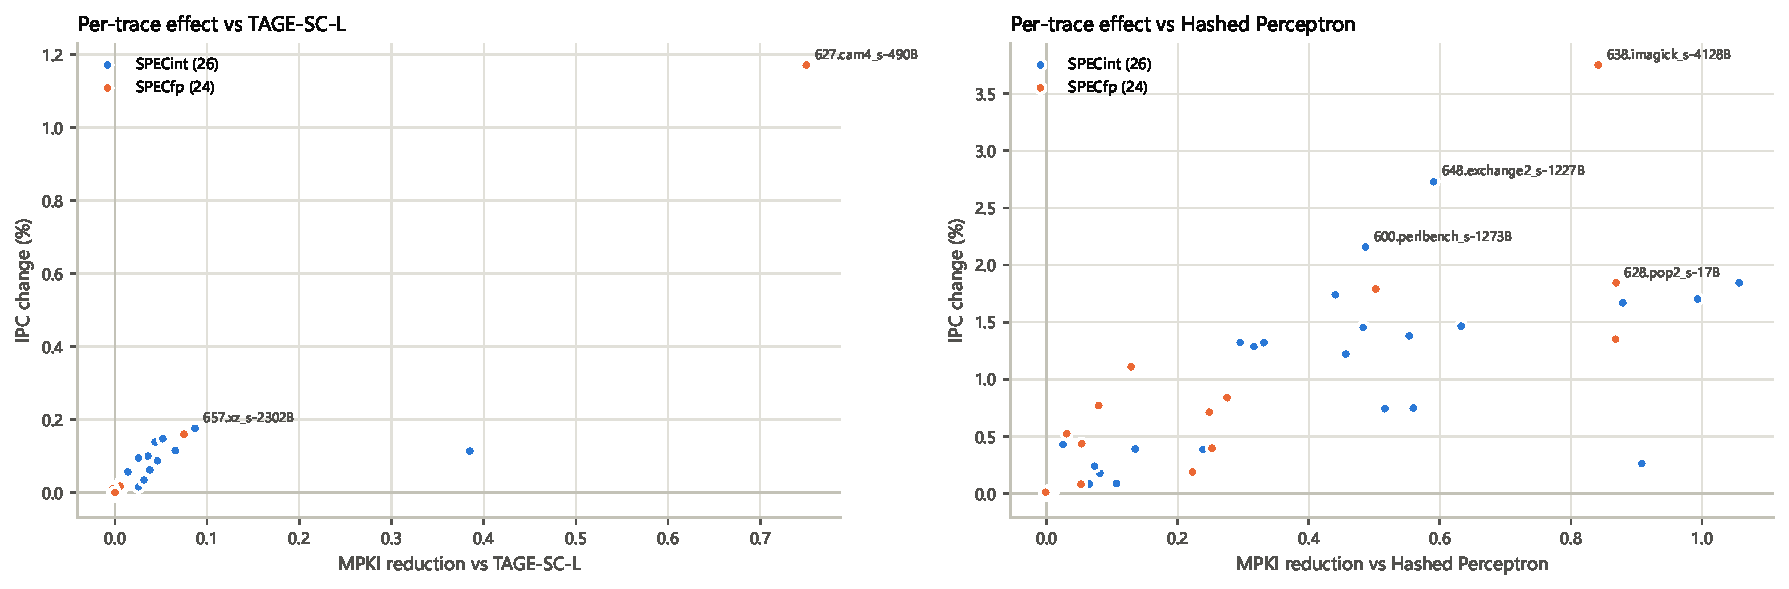
\includegraphics[width=\linewidth]{figures/fig9_mpki_reduction_vs_ipc_gain.pdf}
\caption{Per-trace MPKI reduction against IPC change of \prop{}, coloured by suite; the traces with the largest IPC change are labelled (labels that would overlap are omitted).}\label{fig:mpki_ipc}
\end{figure}

Figure~\ref{fig:mpki_ipc} relates the per-trace MPKI reduction to the per-trace IPC change. Fewer mispredictions never cost measurable performance: no trace loses more than 0.1\% IPC against any baseline. How much IPC an avoided misprediction buys, however, varies widely between traces.
\begin{itemize}
\item \textbf{Relative to the hashed perceptron}, IPC gain grows roughly with MPKI reduction, but with large scatter. On \val{vs_hp_best_trace} a reduction of 0.84 MPKI gives \val{vs_hp_best_pct}\% IPC. Several SPECint traces with a similar or larger reduction gain about half as much.
\item \textbf{Relative to TAGE-SC-L}, 627.cam4\_s-490B stands out (\val{vs_tsl_bestm} MPKI, \val{vs_tsl_best_pct}\% IPC). On \val{tsl_rel1_trace}, by contrast, MPKI falls by \val{tsl_rel1_pct}\% but IPC rises by only \val{tsl_rel1_ipc}\%.
\end{itemize}

The reason is the cost of a misprediction in this simulator. Fetch stops until the mispredicted branch executes, so the penalty depends on how long the branch waits for its operands, and on whether the pipeline is stalled on memory anyway. On 602.gcc\_s-2226B the IPC with \prop{} is only \val{tsl_rel1_prop_ipc}: the core spends most of its time waiting for cache misses, and removing mispredictions recovers little. On compute-bound traces with high IPC, a misprediction wastes a full window of useful work, and the same MPKI reduction is worth more.

For this reason the report gives both MPKI (a property of the predictor) and IPC (its effect on this particular core), and uses the geometric mean for IPC.


\subsection{Simulation runtime}

\begin{table}[H]
\centering\small
\caption{Simulation wall time per run (14 runs in parallel on 8 physical cores, so per-run times include contention).}\label{tab:runtime}
% generated by experiments/scripts/make_report_50trace.py -- do not edit
\begin{tabular}{lrrrr}
\toprule
Predictor & Runs ok & Mean wall time (min) & Max wall time (min) & Total (CPU-h) \\
\midrule
Bimodal & 50/50 & 28.8 & 310.8 & 24.0 \\
Gshare & 50/50 & 29.5 & 312.0 & 24.6 \\
Perceptron & 50/50 & 29.8 & 317.2 & 24.8 \\
Hashed perceptron & 50/50 & 30.6 & 317.6 & 25.5 \\
TAGE & 50/50 & 30.8 & 317.3 & 25.6 \\
TAGE-SC-L & 50/50 & 30.8 & 317.5 & 25.7 \\
TFL-TAGE-SC-L & 50/50 & 30.9 & 317.5 & 25.7 \\
\bottomrule
\end{tabular}

\end{table}

Total simulation effort was \val{total_sim_hours} CPU-hours of wall-clock time per job summed over the \val{n_runs_ok} successful runs. Runtime reflects simulation cost, not predictor latency: ChampSim does not model predictor access time.

% ---------------------------------------------------------------------------------------
\section{Discussion}\label{sec:discussion}
\paragraph{Which predictor is best?} On these \val{n_traces} traces \prop{} is the best of the seven predictors on every aggregate metric: geometric-mean IPC, arithmetic-mean IPC, pooled accuracy and mean MPKI. It is the sole best or tied on \val{n_best_mpki_prop} traces by mispredictions. The margin over the strongest predictor shipped with ChampSim is clear and broad. Relative to the hashed perceptron:
\begin{itemize}
\item mean MPKI is \val{vs_hp_pct_mpki}\% lower, and geometric-mean IPC \val{vs_hp_ipc}\% higher;
\item \prop{} has fewer mispredictions on \val{vs_hp_mpki_win} of \val{n_traces} traces, and no trace loses more than \val{vs_hp_worst_pct}\% IPC;
\item it uses slightly less storage.
\end{itemize}
This is the main result of the evaluation, and it is a property of the TAGE-SC-L design as a whole. Our TAGE-SC-L without the contribution already has no more mispredictions than the hashed perceptron on any trace.

\paragraph{What does the contribution add?} The loop-structure components made possible by the target-free inference reduce mean MPKI by \val{vs_tsl_pct_mpki}\% relative to the same predictor without them. They improve geometric-mean IPC by \val{vs_tsl_ipc}\%. This is a small effect, and three facts qualify it:
\begin{itemize}
\item It is unevenly distributed: one trace (627.cam4\_s-490B) provides \val{vs_tsl_top_share}\% of the MPKI reduction, and the median per-trace IPC change is \val{vs_tsl_median_ipc}\%.
\item It is consistent in sign but not universal: fewer mispredictions on \val{vs_tsl_mpki_win} traces and more on \val{vs_tsl_mpki_loss}, every increase being at most \val{vs_tsl_worstm} MPKI.
\item It costs \val{prop_minus_tsl_pct}\% more storage, and a storage-matched TAGE-SC-L was not evaluated.
\end{itemize}
The aggregate IPC gain of \val{vs_tsl_ipc}\% is more than ten times the largest run-to-run variation measured in the earlier study (at most 0.003\% of geometric-mean IPC when the predictor's random seed is changed). That variation was measured on the original ten traces only, and with a single deterministic run per trace no statistical significance is claimed. The fair summary is that the components work as intended and help clearly on a few programs (627.cam4, 602.gcc, 657.xz). On most other programs they change little, so they are a refinement of TAGE-SC-L rather than a step beyond it. Which loop structures in these programs are responsible was not analysed.

\paragraph{Does the result generalise?} Yes, in direction and ranking. On the \val{n_add} traces never used during design, \prop{} again has the lowest MPKI and the highest geometric-mean IPC, and its relative gains are larger than on the original ten. The IPC gain over TAGE-SC-L is practically the same in both subsets (\val{original10_tsl_ipcimp}\% and \val{additional40_tsl_ipcimp}\%). The larger set also corrects a conclusion of the earlier study, which was based on the original ten traces. On those traces our TAGE was slightly worse than the hashed perceptron. Over all \val{n_traces} traces TAGE is better (\val{tage_mpki} against \val{hp_mpki} MPKI), and is worse on only \val{n_tage_worse_hp} traces.

\paragraph{Arithmetic versus geometric means.} Both means give the same ranking of all seven predictors. The relative differences between the top predictors are also similar under both: \val{vs_tsl_meanipc}\% (arithmetic) against \val{vs_tsl_ipc}\% (geometric) relative to TAGE-SC-L, and \val{vs_hp_meanipc}\% against \val{vs_hp_ipc}\% relative to the hashed perceptron. The conclusions therefore do not depend on the choice of mean.

\paragraph{Practical significance.} For a designer choosing among the predictors shipped with ChampSim, the \val{vs_hp_ipc}\% IPC improvement over the hashed perceptron at slightly lower storage is the practically relevant result. The further \val{vs_tsl_ipc}\% over TAGE-SC-L would justify its cost in a real design only if it were confirmed on a wider workload set. It would also need to be compared against the same storage spent on larger tables. In a processor with wrong-path fetch, the inference would further require checkpointing and repair of the loop-structure state.


% ---------------------------------------------------------------------------------------
\section{Relation to the earlier 10-trace study}\label{sec:previous}
The earlier study evaluated the same predictor on the ten original traces with the same window and simulator configuration; its report, figures, workbook and audit are preserved unchanged in \code{archive/10trace\_study/}.

The new experiment re-simulated the original ten traces from scratch rather than reusing the old outputs, with newly built binaries (a different compiler version) and the trace files from Zenodo. For these \val{orig_identical} predictor--trace combinations the new runs are \emph{identical} to the earlier study in both cycle and misprediction counts (\val{orig_different} differ). The original-10 rows of Table~\ref{tab:subsets} are therefore exactly the earlier study's values, now measured again, while every aggregate quoted elsewhere in this report is over all \val{n_traces_agg} traces. The earlier ablation study (functional replay harness) and its exploration results were not repeated; they are reported only in the archived report.


% ---------------------------------------------------------------------------------------
\section{Limitations and threats to validity}
\begin{itemize}
\item \textbf{Workloads.} \val{n_traces} SimPoint windows of \val{n_bench} SPEC CPU2017 speed benchmarks, 200M measured instructions each. Several benchmarks contribute three or four windows, so they carry more weight in the means than benchmarks with one window. Other suites (server, mobile, CBP traces) were not evaluated.
\item \textbf{Statistics.} One deterministic simulation per predictor and trace. No claim of statistical significance is made; per-trace win/loss counts describe these runs, not a population. The earlier study measured run-to-run noise by changing the predictor's random seed: the standard deviation of mean MPKI was at most 0.03\% of the mean (replay harness), and a different seed moved a design's geometric-mean IPC by at most 0.003\% in ChampSim. Differences of that size should be read as noise.
\item \textbf{Tuning.} The design was tuned on a different window (instructions 1000M--1150M) of the original ten programs, and its final configuration was also checked on the reported window of those ten traces. The \val{n_add} additional traces were never used for tuning; they are the cleaner test of generalisation (Section~\ref{sec:generalisation}).
\item \textbf{Simulator.} ChampSim 2021: direction prediction only, immediate predictor update, no wrong-path execution, no BTB or indirect-target modelling; all branch types count in accuracy and MPKI. Absolute values are not comparable with newer ChampSim versions or with CBP results.
\item \textbf{Inference.} The backward-branch inference is exact only because this ChampSim presents every branch in program order without wrong-path fetch; a speculative front end would need checkpointing and repair of the loop-structure state.
\item \textbf{Re-implementation.} Our TAGE-SC-L (12 tagged tables, about 58 KB) is not Seznec's championship code; no claim is made relative to published state-of-the-art predictors evaluated on other simulators, traces or budgets.
\item \textbf{Storage} is a logical bit count; the hashed perceptron's threshold width is an assumption. Area, energy and access latency were not modelled.
\end{itemize}


% ---------------------------------------------------------------------------------------
\section{Conclusion and future work}
\prop{} was evaluated, unchanged from its frozen design, on \val{n_traces} SPEC CPU2017 traces against all four predictors shipped with ChampSim and against our own TAGE and TAGE-SC-L. All \val{n_runs} simulations succeeded and passed the consistency checks.
\begin{itemize}
\item \textbf{Best overall.} \prop{} is the best of the seven predictors in geometric-mean IPC (\val{prop_gm_ipc}), pooled accuracy (\val{prop_acc}\%) and mean MPKI (\val{prop_mpki}).
\item \textbf{Against the best ChampSim predictor.} Relative to the 64 KB hashed perceptron, \prop{} lowers mean MPKI by \val{vs_hp_pct_mpki}\% and raises geometric-mean IPC by \val{vs_hp_ipc}\%, with fewer mispredictions on \val{vs_hp_mpki_win} of \val{n_traces} traces and slightly less storage. Against the 4 KB default predictors the gains are \val{vs_perc_ipc}\% to \val{vs_bim_ipc}\% in geometric-mean IPC.
\item \textbf{The contribution itself.} Relative to the same TAGE-SC-L without them, the target-free loop-structure components lower mean MPKI by \val{vs_tsl_pct_mpki}\% and raise geometric-mean IPC by \val{vs_tsl_ipc}\%, for \val{prop_minus_tsl_pct}\% more storage. They have fewer mispredictions on \val{vs_tsl_mpki_win} traces and more on \val{vs_tsl_mpki_loss}, and \val{vs_tsl_top_share}\% of the MPKI gain comes from one trace. The contribution is real on these runs but small.
\item \textbf{Generalisation.} The first place of \prop{} and the direction of every one of its gains, observed on the original ten traces, hold on the \val{n_add} traces not used during design.
\end{itemize}

\paragraph{Future work.} Four follow-ups address the open questions of this evaluation:
\begin{itemize}
\item a storage-matched TAGE-SC-L (the \val{prop_minus_tsl_kb} KB spent on larger tables), to separate the value of the loop-structure history from the value of extra storage;
\item an analysis of which loop structures produce the large gains on 627.cam4 and 602.gcc, and why some traces lose a few hundred predictions;
\item evaluation on non-SPEC workloads (server, CBP and mobile traces) and in a ChampSim version with wrong-path execution, where the inference needs repair after mispredictions;
\item modelling the access latency of the larger corrector, which this simulator does not capture.
\end{itemize}


\bibliographystyle{plainnat}
\bibliography{references}

\appendix
\section{IPC, MPKI and accuracy of every predictor on every trace}\label{app:all}
{\footnotesize\setlength{\tabcolsep}{4pt}% generated by experiments/scripts/make_report_50trace.py -- do not edit
\begin{longtable}{lrrrrrrr}
\caption{IPC of every predictor on every trace. Bim.\ = bimodal, Perc.\ = perceptron, Hashed P.\ = hashed perceptron, TSL = TAGE-SC-L, Proposed = TFL-TAGE-SC-L; bold = best on the trace.}\label{tab:ipc_all}\\
\toprule
Trace & Bim. & Gshare & Perc. & Hashed P. & TAGE & TSL & Proposed \\
\midrule
\endhead
600.perlbench\_s-1273B & 1.3808 & 1.4042 & 1.4339 & 1.4895 & 1.5186 & 1.5215 & \textbf{1.5216} \\
600.perlbench\_s-210B & 1.3853 & 1.4092 & 1.4781 & 1.5412 & 1.5591 & 1.5612 & \textbf{1.5616} \\
600.perlbench\_s-570B & 0.8886 & 0.8925 & 0.9088 & 0.9951 & 1.0081 & \textbf{1.0096} & 1.0095 \\
602.gcc\_s-1850B & 0.2809 & 0.3178 & 0.3190 & 0.3470 & 0.3471 & 0.3471 & \textbf{0.3473} \\
602.gcc\_s-2226B & 0.1073 & 0.1079 & 0.1080 & 0.1082 & 0.1083 & 0.1083 & \textbf{0.1085} \\
602.gcc\_s-734B & 0.4370 & 0.5226 & 0.5229 & 0.5280 & 0.5286 & 0.5290 & \textbf{0.5290} \\
603.bwaves\_s-1080B & 1.1996 & 1.3123 & 1.2971 & 1.5314 & 1.5409 & 1.5431 & \textbf{1.5432} \\
603.bwaves\_s-2609B & 0.7288 & 0.7301 & 0.7351 & 0.7351 & 0.7351 & \textbf{0.7351} & 0.7351 \\
603.bwaves\_s-891B & 0.4920 & 0.5391 & 0.5391 & 0.5391 & 0.5391 & \textbf{0.5401} & 0.5401 \\
605.mcf\_s-1152B & 0.2908 & 0.2883 & 0.3032 & 0.3122 & 0.3073 & 0.3122 & \textbf{0.3124} \\
605.mcf\_s-1536B & 0.1504 & 0.1505 & 0.1505 & 0.1505 & 0.1505 & \textbf{0.1505} & 0.1505 \\
605.mcf\_s-472B & 0.2762 & 0.2759 & 0.2769 & 0.2916 & 0.2904 & 0.2923 & \textbf{0.2923} \\
607.cactuBSSN\_s-2421B & 1.1950 & 1.1952 & 1.1952 & 1.1953 & 1.1954 & \textbf{1.1955} & 1.1955 \\
607.cactuBSSN\_s-3477B & 1.1688 & 1.1688 & 1.1688 & \textbf{1.1689} & 1.1688 & 1.1688 & 1.1688 \\
619.lbm\_s-2676B & 0.6331 & 0.6331 & 0.6331 & 0.6331 & \textbf{0.6332} & 0.6331 & 0.6330 \\
619.lbm\_s-3766B & 0.4689 & 0.4689 & 0.4689 & 0.4689 & 0.4689 & 0.4689 & \textbf{0.4689} \\
620.omnetpp\_s-141B & 0.3119 & 0.3234 & 0.3310 & 0.3388 & 0.3391 & 0.3408 & \textbf{0.3413} \\
620.omnetpp\_s-874B & 0.3361 & 0.3468 & 0.3542 & 0.3595 & 0.3597 & 0.3619 & \textbf{0.3622} \\
621.wrf\_s-575B & 1.1071 & 1.1297 & 1.1615 & 1.1839 & 1.1879 & 1.1886 & \textbf{1.1886} \\
621.wrf\_s-6673B & 0.7895 & 0.7914 & 0.7948 & 0.7968 & 0.7974 & \textbf{0.7976} & 0.7975 \\
621.wrf\_s-8100B & 1.1458 & 1.1788 & 1.1897 & 1.2101 & 1.2113 & 1.2168 & \textbf{1.2187} \\
623.xalancbmk\_s-10B & 0.2911 & 0.3136 & 0.3156 & 0.3217 & 0.3229 & 0.3230 & \textbf{0.3230} \\
623.xalancbmk\_s-165B & 0.5531 & 0.5652 & 0.7183 & 0.7205 & 0.7207 & \textbf{0.7207} & 0.7207 \\
625.x264\_s-12B & 1.5491 & 1.7205 & 1.7567 & 1.7761 & 1.7832 & \textbf{1.7839} & 1.7838 \\
625.x264\_s-18B & 1.4318 & 1.5470 & 1.5738 & 1.6081 & 1.6085 & 1.6140 & \textbf{1.6144} \\
627.cam4\_s-490B & 0.9434 & 1.0209 & 1.0305 & 1.0359 & 1.0326 & 1.0377 & \textbf{1.0499} \\
627.cam4\_s-573B & 1.0529 & 1.1215 & 1.1426 & 1.2081 & 1.2272 & 1.2297 & \textbf{1.2298} \\
628.pop2\_s-17B & 1.1552 & 1.1633 & 1.1668 & 1.2095 & 1.2285 & 1.2316 & \textbf{1.2318} \\
631.deepsjeng\_s-928B & 0.9633 & 1.0510 & 1.0708 & 1.1778 & 1.1771 & 1.1904 & \textbf{1.1922} \\
638.imagick\_s-4128B & 1.7865 & 1.7977 & 1.7977 & 1.8014 & 1.8677 & \textbf{1.8689} & 1.8689 \\
638.imagick\_s-824B & 1.2097 & 1.2117 & 1.2100 & 1.2139 & 1.2139 & \textbf{1.2140} & 1.2139 \\
641.leela\_s-149B & 0.7501 & 0.7652 & 0.7974 & 0.8702 & 0.8740 & 0.8848 & \textbf{0.8850} \\
641.leela\_s-334B & 0.7381 & 0.7763 & 0.7975 & 0.9083 & 0.9134 & 0.9229 & \textbf{0.9234} \\
641.leela\_s-602B & 0.7194 & 0.7422 & 0.7673 & 0.8485 & 0.8544 & 0.8638 & \textbf{0.8641} \\
644.nab\_s-5853B & 1.1942 & 1.3427 & 1.3426 & 1.3430 & 1.3430 & \textbf{1.3431} & 1.3431 \\
644.nab\_s-7928B & 1.2058 & 1.2077 & 1.2114 & 1.2122 & 1.2119 & \textbf{1.2124} & 1.2124 \\
644.nab\_s-9322B & 1.0587 & 1.0606 & 1.0654 & 1.0667 & 1.0657 & \textbf{1.0668} & 1.0667 \\
648.exchange2\_s-1227B & 1.2632 & 1.6124 & 1.7149 & 1.8981 & 1.9298 & 1.9494 & \textbf{1.9499} \\
648.exchange2\_s-1712B & 1.3765 & 1.7710 & 1.9031 & 2.0936 & 2.1120 & 2.1211 & \textbf{2.1212} \\
648.exchange2\_s-210B & 1.3171 & 1.7089 & 1.8339 & 2.0758 & 2.0884 & 2.1013 & \textbf{2.1025} \\
648.exchange2\_s-584B & 1.2775 & 1.6481 & 1.7480 & 1.9857 & 2.0045 & 2.0182 & \textbf{2.0202} \\
649.fotonik3d\_s-1176B & \textbf{0.6074} & 0.6074 & 0.6074 & 0.6074 & 0.6074 & 0.6074 & 0.6074 \\
649.fotonik3d\_s-1B & 0.9909 & 1.1307 & 1.1641 & 1.2118 & 1.2214 & \textbf{1.2220} & 1.2220 \\
649.fotonik3d\_s-7084B & 0.5978 & 0.5978 & 0.5978 & \textbf{0.5978} & 0.5978 & 0.5978 & 0.5978 \\
654.roms\_s-1021B & 0.9792 & 1.2914 & 1.3217 & 1.4625 & 1.4670 & \textbf{1.4787} & 1.4787 \\
654.roms\_s-293B & 0.9643 & 0.9644 & 0.9644 & 0.9643 & 0.9645 & \textbf{0.9694} & 0.9694 \\
654.roms\_s-842B & 1.0134 & 1.5824 & 1.6398 & 1.7431 & 1.7507 & 1.7507 & \textbf{1.7508} \\
657.xz\_s-2302B & 0.8823 & 0.9156 & 0.9283 & 0.9851 & 0.9769 & 0.9969 & \textbf{0.9987} \\
657.xz\_s-3167B & 1.0146 & 1.0327 & 1.0420 & 1.1151 & 1.1181 & 1.1301 & \textbf{1.1314} \\
657.xz\_s-56B & 1.6649 & 1.6679 & 1.7011 & \textbf{1.7072} & 1.7072 & 1.7072 & 1.7072 \\
\bottomrule
\end{longtable}
}
{\footnotesize\setlength{\tabcolsep}{4pt}% generated by experiments/scripts/make_report_50trace.py -- do not edit
\begin{longtable}{lrrrrrrr}
\caption{MPKI of every predictor on every trace. Bim.\ = bimodal, Perc.\ = perceptron, Hashed P.\ = hashed perceptron, TSL = TAGE-SC-L, Proposed = TFL-TAGE-SC-L; bold = best on the trace.}\label{tab:mpki_all}\\
\toprule
Trace & Bim. & Gshare & Perc. & Hashed P. & TAGE & TSL & Proposed \\
\midrule
\endhead
600.perlbench\_s-1273B & 2.996 & 2.482 & 1.917 & 1.120 & 0.678 & 0.635 & \textbf{0.634} \\
600.perlbench\_s-210B & 3.352 & 2.993 & 1.775 & 0.954 & 0.696 & 0.666 & \textbf{0.659} \\
600.perlbench\_s-570B & 6.159 & 5.982 & 5.243 & 1.534 & 1.107 & \textbf{1.051} & 1.051 \\
602.gcc\_s-1850B & 19.830 & 9.062 & 8.737 & 0.097 & 0.065 & 0.063 & \textbf{0.032} \\
602.gcc\_s-2226B & 3.119 & 1.831 & 1.562 & 1.057 & 0.554 & 0.534 & \textbf{0.149} \\
602.gcc\_s-734B & 12.790 & 0.899 & 0.855 & 0.235 & 0.197 & 0.155 & \textbf{0.153} \\
603.bwaves\_s-1080B & 18.076 & 9.467 & 11.711 & 0.094 & 0.035 & \textbf{0.014} & 0.015 \\
603.bwaves\_s-2609B & 4.685 & 0.787 & 0.007 & 0.007 & 0.007 & \textbf{0.000} & 0.000 \\
603.bwaves\_s-891B & 24.103 & 0.223 & 0.223 & 0.223 & 0.223 & 0.000 & \textbf{0.000} \\
605.mcf\_s-1152B & 21.058 & 17.734 & 15.850 & 13.981 & 14.537 & 13.920 & \textbf{13.874} \\
605.mcf\_s-1536B & 0.035 & 0.019 & 0.019 & 0.019 & 0.011 & \textbf{0.011} & 0.011 \\
605.mcf\_s-472B & 1.826 & 1.682 & 1.596 & 1.106 & 1.117 & 1.033 & \textbf{1.033} \\
607.cactuBSSN\_s-2421B & 0.013 & 0.009 & 0.007 & 0.007 & 0.005 & \textbf{0.003} & 0.003 \\
607.cactuBSSN\_s-3477B & 0.003 & 0.001 & 0.002 & 0.001 & 0.001 & \textbf{0.000} & 0.000 \\
619.lbm\_s-2676B & 0.211 & 0.116 & 0.114 & 0.109 & 0.101 & \textbf{0.101} & 0.101 \\
619.lbm\_s-3766B & 0.632 & 0.402 & 0.373 & 0.366 & 0.374 & \textbf{0.365} & 0.367 \\
620.omnetpp\_s-141B & 10.695 & 8.258 & 5.855 & 3.838 & 3.722 & 3.322 & \textbf{3.278} \\
620.omnetpp\_s-874B & 8.732 & 6.953 & 4.975 & 3.727 & 3.665 & 3.237 & \textbf{3.211} \\
621.wrf\_s-575B & 5.341 & 3.189 & 1.519 & 0.475 & 0.263 & 0.224 & \textbf{0.223} \\
621.wrf\_s-6673B & 1.901 & 1.277 & 0.389 & 0.079 & 0.044 & \textbf{0.026} & 0.027 \\
621.wrf\_s-8100B & 4.247 & 2.321 & 1.832 & 1.166 & 1.146 & 0.993 & \textbf{0.918} \\
623.xalancbmk\_s-10B & 12.889 & 2.576 & 2.042 & 0.692 & 0.478 & 0.455 & \textbf{0.453} \\
623.xalancbmk\_s-165B & 10.298 & 7.723 & 0.141 & 0.031 & 0.021 & \textbf{0.020} & 0.020 \\
625.x264\_s-12B & 4.694 & 0.670 & 0.496 & 0.079 & 0.057 & \textbf{0.053} & 0.054 \\
625.x264\_s-18B & 4.597 & 1.660 & 1.289 & 0.662 & 0.620 & 0.533 & \textbf{0.527} \\
627.cam4\_s-490B & 11.935 & 5.741 & 5.101 & 4.696 & 4.904 & 4.578 & \textbf{3.828} \\
627.cam4\_s-573B & 8.469 & 3.875 & 3.154 & 0.980 & 0.549 & 0.484 & \textbf{0.478} \\
628.pop2\_s-17B & 3.713 & 3.258 & 3.065 & 1.197 & 0.450 & 0.333 & \textbf{0.328} \\
631.deepsjeng\_s-928B & 13.746 & 9.760 & 8.481 & 4.166 & 4.194 & 3.761 & \textbf{3.709} \\
638.imagick\_s-4128B & 1.707 & 0.889 & 0.889 & 0.842 & 0.023 & \textbf{0.000} & 0.000 \\
638.imagick\_s-824B & 0.317 & 0.190 & 0.274 & 0.090 & 0.088 & \textbf{0.088} & 0.089 \\
641.leela\_s-149B & 20.586 & 19.217 & 16.332 & 10.929 & 10.678 & 9.962 & \textbf{9.936} \\
641.leela\_s-334B & 20.545 & 17.273 & 15.340 & 8.304 & 7.972 & 7.463 & \textbf{7.425} \\
641.leela\_s-602B & 20.509 & 18.606 & 16.052 & 10.043 & 9.614 & 9.018 & \textbf{8.986} \\
644.nab\_s-5853B & 2.804 & 0.028 & 0.033 & 0.015 & 0.012 & \textbf{0.011} & 0.011 \\
644.nab\_s-7928B & 1.770 & 1.677 & 1.550 & 1.488 & 1.537 & \textbf{1.484} & 1.486 \\
644.nab\_s-9322B & 2.486 & 2.387 & 2.205 & 2.118 & 2.190 & \textbf{2.117} & 2.120 \\
648.exchange2\_s-1227B & 21.539 & 6.823 & 4.518 & 1.372 & 1.009 & 0.791 & \textbf{0.782} \\
648.exchange2\_s-1712B & 19.997 & 5.838 & 3.366 & 0.721 & 0.498 & 0.391 & \textbf{0.389} \\
648.exchange2\_s-210B & 22.410 & 6.879 & 4.366 & 0.822 & 0.668 & 0.520 & \textbf{0.506} \\
648.exchange2\_s-584B & 22.621 & 7.332 & 5.034 & 1.228 & 0.998 & 0.823 & \textbf{0.787} \\
649.fotonik3d\_s-1176B & \textbf{0.004} & 0.004 & 0.004 & 0.004 & 0.004 & 0.004 & 0.004 \\
649.fotonik3d\_s-1B & 9.174 & 4.163 & 1.722 & 0.277 & 0.037 & \textbf{0.001} & 0.001 \\
649.fotonik3d\_s-7084B & 0.056 & 0.056 & 0.056 & 0.000 & \textbf{0.000} & 0.000 & 0.000 \\
654.roms\_s-1021B & 24.894 & 2.938 & 2.503 & 0.130 & 0.092 & \textbf{0.001} & 0.001 \\
654.roms\_s-293B & 0.033 & 0.032 & 0.032 & 0.032 & 0.021 & 0.001 & \textbf{0.001} \\
654.roms\_s-842B & 28.051 & 1.505 & 0.725 & 0.105 & 0.053 & 0.052 & \textbf{0.052} \\
657.xz\_s-2302B & 15.390 & 13.153 & 11.979 & 9.417 & 9.705 & 8.950 & \textbf{8.863} \\
657.xz\_s-3167B & 11.045 & 10.569 & 9.502 & 5.445 & 5.232 & 4.878 & \textbf{4.813} \\
657.xz\_s-56B & 0.628 & 0.418 & 0.209 & \textbf{0.000} & 0.000 & 0.000 & 0.000 \\
\bottomrule
\end{longtable}
}
{\footnotesize\setlength{\tabcolsep}{4pt}% generated by experiments/scripts/make_report_50trace.py -- do not edit
\begin{longtable}{lrrrrrrr}
\caption{Branch prediction accuracy (\%, all branch types) of every predictor on every trace. Bim.\ = bimodal, Perc.\ = perceptron, Hashed P.\ = hashed perceptron, TSL = TAGE-SC-L, Proposed = TFL-TAGE-SC-L; bold = best on the trace.}\label{tab:acc_all}\\
\toprule
Trace & Bim. & Gshare & Perc. & Hashed P. & TAGE & TSL & Proposed \\
\midrule
\endhead
600.perlbench\_s-1273B & 97.861 & 98.228 & 98.632 & 99.200 & 99.516 & 99.547 & \textbf{99.548} \\
600.perlbench\_s-210B & 97.607 & 97.864 & 98.733 & 99.319 & 99.503 & 99.525 & \textbf{99.530} \\
600.perlbench\_s-570B & 96.264 & 96.372 & 96.820 & 99.069 & 99.328 & \textbf{99.363} & 99.362 \\
602.gcc\_s-1850B & 92.266 & 96.466 & 96.592 & 99.962 & 99.975 & 99.975 & \textbf{99.988} \\
602.gcc\_s-2226B & 99.125 & 99.486 & 99.562 & 99.703 & 99.845 & 99.850 & \textbf{99.958} \\
602.gcc\_s-734B & 94.674 & 99.626 & 99.644 & 99.902 & 99.918 & 99.935 & \textbf{99.936} \\
603.bwaves\_s-1080B & 87.561 & 93.485 & 91.941 & 99.935 & 99.976 & \textbf{99.990} & 99.990 \\
603.bwaves\_s-2609B & 81.232 & 96.848 & 99.971 & 99.971 & 99.971 & \textbf{100.000} & 100.000 \\
603.bwaves\_s-891B & 85.619 & 99.867 & 99.867 & 99.867 & 99.867 & 100.000 & \textbf{100.000} \\
605.mcf\_s-1152B & 91.852 & 93.138 & 93.867 & 94.590 & 94.375 & 94.614 & \textbf{94.631} \\
605.mcf\_s-1536B & 99.978 & 99.988 & 99.988 & 99.988 & 99.993 & \textbf{99.993} & 99.993 \\
605.mcf\_s-472B & 98.583 & 98.695 & 98.762 & 99.142 & 99.134 & 99.198 & \textbf{99.199} \\
607.cactuBSSN\_s-2421B & 99.039 & 99.356 & 99.483 & 99.530 & 99.662 & \textbf{99.790} & 99.787 \\
607.cactuBSSN\_s-3477B & 99.962 & 99.986 & 99.982 & 99.987 & 99.985 & \textbf{99.998} & 99.997 \\
619.lbm\_s-2676B & 98.257 & 99.043 & 99.055 & 99.097 & 99.162 & \textbf{99.165} & 99.163 \\
619.lbm\_s-3766B & 95.949 & 97.427 & 97.612 & 97.656 & 97.604 & \textbf{97.661} & 97.647 \\
620.omnetpp\_s-141B & 94.906 & 96.067 & 97.211 & 98.172 & 98.227 & 98.418 & \textbf{98.439} \\
620.omnetpp\_s-874B & 95.802 & 96.658 & 97.609 & 98.208 & 98.238 & 98.444 & \textbf{98.456} \\
621.wrf\_s-575B & 96.015 & 97.621 & 98.866 & 99.645 & 99.804 & 99.833 & \textbf{99.833} \\
621.wrf\_s-6673B & 96.839 & 97.877 & 99.352 & 99.868 & 99.926 & \textbf{99.957} & 99.956 \\
621.wrf\_s-8100B & 96.558 & 98.119 & 98.515 & 99.055 & 99.071 & 99.195 & \textbf{99.256} \\
623.xalancbmk\_s-10B & 95.018 & 99.004 & 99.211 & 99.733 & 99.815 & 99.824 & \textbf{99.825} \\
623.xalancbmk\_s-165B & 96.291 & 97.218 & 99.949 & 99.989 & 99.993 & \textbf{99.993} & 99.993 \\
625.x264\_s-12B & 88.925 & 98.420 & 98.831 & 99.814 & 99.865 & \textbf{99.875} & 99.874 \\
625.x264\_s-18B & 90.214 & 96.467 & 97.256 & 98.591 & 98.680 & 98.866 & \textbf{98.879} \\
627.cam4\_s-490B & 87.572 & 94.022 & 94.688 & 95.110 & 94.893 & 95.233 & \textbf{96.014} \\
627.cam4\_s-573B & 93.655 & 97.097 & 97.637 & 99.266 & 99.588 & 99.638 & \textbf{99.642} \\
628.pop2\_s-17B & 97.565 & 97.863 & 97.989 & 99.215 & 99.705 & 99.781 & \textbf{99.785} \\
631.deepsjeng\_s-928B & 90.656 & 93.365 & 94.235 & 97.168 & 97.149 & 97.443 & \textbf{97.479} \\
638.imagick\_s-4128B & 99.118 & 99.541 & 99.541 & 99.565 & 99.988 & \textbf{100.000} & 100.000 \\
638.imagick\_s-824B & 99.803 & 99.882 & 99.830 & 99.944 & 99.945 & \textbf{99.945} & 99.945 \\
641.leela\_s-149B & 87.561 & 88.388 & 90.131 & 93.396 & 93.548 & 93.980 & \textbf{93.996} \\
641.leela\_s-334B & 88.177 & 90.061 & 91.173 & 95.222 & 95.412 & 95.706 & \textbf{95.727} \\
641.leela\_s-602B & 87.950 & 89.068 & 90.569 & 94.099 & 94.351 & 94.702 & \textbf{94.720} \\
644.nab\_s-5853B & 97.103 & 99.971 & 99.966 & 99.984 & 99.987 & \textbf{99.988} & 99.988 \\
644.nab\_s-7928B & 98.155 & 98.252 & 98.385 & 98.449 & 98.398 & \textbf{98.453} & 98.451 \\
644.nab\_s-9322B & 98.069 & 98.146 & 98.287 & 98.355 & 98.299 & \textbf{98.356} & 98.354 \\
648.exchange2\_s-1227B & 84.920 & 95.223 & 96.837 & 99.039 & 99.294 & 99.446 & \textbf{99.453} \\
648.exchange2\_s-1712B & 85.089 & 95.647 & 97.490 & 99.463 & 99.628 & 99.709 & \textbf{99.710} \\
648.exchange2\_s-210B & 83.549 & 94.950 & 96.795 & 99.396 & 99.509 & 99.618 & \textbf{99.629} \\
648.exchange2\_s-584B & 83.921 & 94.788 & 96.422 & 99.127 & 99.290 & 99.415 & \textbf{99.440} \\
649.fotonik3d\_s-1176B & \textbf{99.975} & 99.975 & 99.975 & 99.975 & 99.975 & 99.975 & 99.975 \\
649.fotonik3d\_s-1B & 96.141 & 98.249 & 99.276 & 99.884 & 99.984 & \textbf{99.999} & 99.999 \\
649.fotonik3d\_s-7084B & 99.186 & 99.186 & 99.186 & 99.998 & \textbf{99.999} & 99.999 & 99.999 \\
654.roms\_s-1021B & 83.416 & 98.043 & 98.332 & 99.913 & 99.939 & \textbf{99.999} & 99.999 \\
654.roms\_s-293B & 99.908 & 99.909 & 99.909 & 99.910 & 99.940 & 99.996 & \textbf{99.996} \\
654.roms\_s-842B & 82.939 & 99.085 & 99.559 & 99.936 & 99.968 & 99.968 & \textbf{99.968} \\
657.xz\_s-2302B & 87.690 & 89.479 & 90.419 & 92.468 & 92.237 & 92.841 & \textbf{92.911} \\
657.xz\_s-3167B & 92.557 & 92.878 & 93.597 & 96.331 & 96.474 & 96.713 & \textbf{96.757} \\
657.xz\_s-56B & 96.875 & 97.917 & 98.958 & \textbf{100.000} & 100.000 & 100.000 & 100.000 \\
\bottomrule
\end{longtable}
}

\section{Trace manifest}\label{app:manifest}
{\small% generated by experiments/scripts/make_report_50trace.py -- do not edit
\begin{longtable}{lllrl}
\caption{Trace manifest: the 50 SPEC CPU2017 traces (Zenodo record 10960004); every file passed \texttt{xz -t} and matches Zenodo's size and MD5. Each trace holds 2,000M instructions.}\label{tab:manifest}\\
\toprule
Trace & Set & Suite & Size (MB) & MD5 (first 12 hex) \\
\midrule
\endhead
602.gcc\_s-1850B & original 10 & INT & 704.8 & \texttt{a01fb04176de} \\
605.mcf\_s-1152B & original 10 & INT & 1,049.2 & \texttt{b2a44b59bbc0} \\
607.cactuBSSN\_s-2421B & original 10 & FP & 257.2 & \texttt{8030545e6ef2} \\
619.lbm\_s-2676B & original 10 & FP & 771.5 & \texttt{840647f7f95b} \\
620.omnetpp\_s-141B & original 10 & INT & 831.6 & \texttt{6cdf4692ff2a} \\
623.xalancbmk\_s-10B & original 10 & INT & 585.1 & \texttt{3b16f6c9d358} \\
625.x264\_s-12B & original 10 & INT & 247.4 & \texttt{9fff2d0c19e2} \\
631.deepsjeng\_s-928B & original 10 & INT & 266.3 & \texttt{823e5fdcf525} \\
638.imagick\_s-824B & original 10 & FP & 59.5 & \texttt{fd4b5a944a45} \\
657.xz\_s-2302B & original 10 & INT & 520.3 & \texttt{4a5c15053d01} \\
600.perlbench\_s-1273B & additional 40 & INT & 145.5 & \texttt{eff9e488f6d5} \\
600.perlbench\_s-210B & additional 40 & INT & 155.4 & \texttt{8ac40f7348a2} \\
600.perlbench\_s-570B & additional 40 & INT & 153.8 & \texttt{1fb27aed6d81} \\
602.gcc\_s-2226B & additional 40 & INT & 872.2 & \texttt{b39ebc6bec73} \\
602.gcc\_s-734B & additional 40 & INT & 368.7 & \texttt{f3b5fb7301a2} \\
603.bwaves\_s-1080B & additional 40 & FP & 39.6 & \texttt{be58dacc1669} \\
603.bwaves\_s-2609B & additional 40 & FP & 386.3 & \texttt{14ac8ffc0a45} \\
603.bwaves\_s-891B & additional 40 & FP & 413.2 & \texttt{8efc36ccea12} \\
605.mcf\_s-1536B & additional 40 & INT & 325.0 & \texttt{73f39eb04b09} \\
605.mcf\_s-472B & additional 40 & INT & 366.3 & \texttt{692697643227} \\
607.cactuBSSN\_s-3477B & additional 40 & FP & 228.2 & \texttt{7d30808db6bc} \\
619.lbm\_s-3766B & additional 40 & FP & 846.4 & \texttt{800972ee67b5} \\
620.omnetpp\_s-874B & additional 40 & INT & 802.3 & \texttt{533f98aefe9d} \\
621.wrf\_s-575B & additional 40 & FP & 352.8 & \texttt{5ec5bd634b05} \\
621.wrf\_s-6673B & additional 40 & FP & 282.0 & \texttt{b3f103221b99} \\
621.wrf\_s-8100B & additional 40 & FP & 275.0 & \texttt{27305ea16679} \\
623.xalancbmk\_s-165B & additional 40 & INT & 143.2 & \texttt{dbc3cb4936d5} \\
625.x264\_s-18B & additional 40 & INT & 246.5 & \texttt{8c2f778998e9} \\
627.cam4\_s-490B & additional 40 & FP & 394.3 & \texttt{4c8247b1ccf2} \\
627.cam4\_s-573B & additional 40 & FP & 151.9 & \texttt{bb01996fa958} \\
628.pop2\_s-17B & additional 40 & FP & 314.0 & \texttt{db580bd8e9ca} \\
638.imagick\_s-4128B & additional 40 & FP & 50.7 & \texttt{ed67c3d3df78} \\
641.leela\_s-149B & additional 40 & INT & 333.5 & \texttt{934f4331c89d} \\
641.leela\_s-334B & additional 40 & INT & 250.4 & \texttt{e955331bff15} \\
641.leela\_s-602B & additional 40 & INT & 307.3 & \texttt{f593fe5bc590} \\
644.nab\_s-5853B & additional 40 & FP & 123.5 & \texttt{617ed8cc9f55} \\
644.nab\_s-7928B & additional 40 & FP & 114.6 & \texttt{f0835acc1b7b} \\
644.nab\_s-9322B & additional 40 & FP & 134.9 & \texttt{a6214cb70a92} \\
648.exchange2\_s-1227B & additional 40 & INT & 70.3 & \texttt{1f8aaf3702c3} \\
648.exchange2\_s-1712B & additional 40 & INT & 50.5 & \texttt{aef8988198e9} \\
648.exchange2\_s-210B & additional 40 & INT & 49.6 & \texttt{01e87200c2c8} \\
648.exchange2\_s-584B & additional 40 & INT & 52.2 & \texttt{4488cd35fe6b} \\
649.fotonik3d\_s-1176B & additional 40 & FP & 328.7 & \texttt{93afa8aeaab7} \\
649.fotonik3d\_s-1B & additional 40 & FP & 25.3 & \texttt{a9ee5d35387f} \\
649.fotonik3d\_s-7084B & additional 40 & FP & 517.4 & \texttt{d56355509b13} \\
654.roms\_s-1021B & additional 40 & FP & 25.6 & \texttt{0039e1b3316c} \\
654.roms\_s-293B & additional 40 & FP & 315.2 & \texttt{b18a970aee84} \\
654.roms\_s-842B & additional 40 & FP & 199.9 & \texttt{f60d65d0fd66} \\
657.xz\_s-3167B & additional 40 & INT & 465.4 & \texttt{cac895d9cebc} \\
657.xz\_s-56B & additional 40 & INT & 93.8 & \texttt{5211b1778f2c} \\
\bottomrule
\end{longtable}
}

\section{Reproduction}\label{app:repro}
The complete procedure is in \code{README.md}. In short (Linux or WSL, with \code{g++}, \code{xz}, \code{python3}):
{\footnotesize
\begin{verbatim}
# 1. traces: download the 50 files of experiments/traces/target_traces.tsv
#    from Zenodo record 10960004 into TRACE_DIR, then verify and map them
experiments/scripts/check_traces.sh TRACE_DIR experiments/traces/trace_integrity.txt
python3 experiments/scripts/reconcile_traces.py --trace-dir TRACE_DIR \
        --check experiments/traces/trace_integrity.txt   # -> trace_manifest.csv, trace_map.tsv
# 2. build the seven binaries
bash experiments/scripts/build_all_50trace.sh
# 3. run the 350 simulations (resumable)
python3 experiments/scripts/run_matrix.py --stage M50_50M_200M \
        --bins bimodal,gshare,perceptron,hashed_perceptron,tage,tsl_base,tsl_proposed \
        --trace-map experiments/traces/trace_map.tsv --warm 50 --sim 200 -j 14
# 4. analysis, figures, report values and PDF
python3 experiments/scripts/analyze_50trace.py
python3 experiments/scripts/make_figures_50trace.py      # needs matplotlib
python3 experiments/scripts/make_report_50trace.py
cd report_50trace && tectonic main.tex
\end{verbatim}
}
The predictor alone can also be built with ChampSim's own script: \code{./build\_champsim.sh tfl\_tage\_scl no no no no lru 1}.


\end{document}
